%*******************************************************************************
%****************************** Third Chapter *********************************
%*******************************************************************************

\chapter{Evaluation of LISP mapping system}
\label{cha:mds_evaluation}

% **************************** Define Graphics Path **************************
\ifpdf
    \graphicspath{{Chapter4/Pics/Raster/}{Chapter4/Pics/PDF/}{Chapter4/}}
\else
    \graphicspath{{Chapter4/Pics/Vector/}{Chapter4/}}
\fi

%-< ABSTRACT >--------------------------------------------------------------------

%-< ABSTRACT >--------------------------------------------------------------------

%\section{Introduction}
%\label{sec:mds_introduction}

%In the LISP architecture, the mapping between RLOCs and EIDs is the cornerstone and a deep study on the performance of LISP mapping system is essential. 
As presented in Chapter~\ref{cha:lisp_overview}, to retrieve the routing information (RLOCs) for EIDs, LISP relies on a pull model by explicitly querying the \acrfull{mds}. The performance of the mapping system is of paramount importance for LISP. Thus, we leverage on \emph{LISP Beta Network}~\cite{lispbeta}, to conduct measurement campaigns about the mapping system. Such a worldwide real playground has been used to assess the state of LISP deployment and evolution over the years~\cite{lispCCR}. Yet, to our best knowledge, nobody at the moment has evaluated the mapping system from the following two standpoints: Stability and Consistency. We thus propose a much deeper study and a more thorough evaluation, focusing on the exploration of all the EID space through active LIG (LISP Internet Groper~\cite{rfc6835}) measurement. The temporal comparison shows that the mapping system is quite stable over time and a crosswise comparison indicates that the mapping system is consistent between network entities. However, some instabilities and inconsistencies are also identified through the evaluation, which indicates that the mapping system can be improved. Besides proposing a brand new taxonomy in order to classify them, we carry out an in-depth investigation of such cases to provide hints on how to improve the performance of LISP.

The remainder of this chapter is organized as follows. Sec.~\ref{sec:mds_methodology} presents an overview of the experiment campaigns and introduces the metrics that we use to evaluate the performance of the mapping system. Sec.~\ref{sec:mds_stability} and Sec.~\ref{sec:mds_consistency} respectively describe the mapping system stability and consistency results in details, as well as the instability and inconsistency cases by using the proposed taxonomy, and investigate in depth the causes from different viewpoints. Finally, Sec.~\ref{sec:mds_conclusion} provides some findings and concludes this chapter.

%-< SECTION >--------------------------------------------------------------------
\section{Methodology}
\label{sec:mds_methodology}
In order to collect data to carry out our analysis, several measurements campaigns have been performed. Hereafter we provide an overview on the measurements and the metrics used in our evaluation.

%-< SUB SECTION >--------------------------------------------------------------------
\subsection{Measurements overview}
\label{sec:mds_overview}
% \begin{itemize}[noitemsep,topsep=0pt]
%     \item The experiments lasted two weeks, from July 2\textsuperscript{nd} to 18\textsuperscript{th} 2013. 
%     \item From a set of different vantage points (VPs).
%     \item Send the Map-Request to all the MRs of the LISP Beta Network by LIG.
%     \item Interval is 30 minutes.
% \end{itemize}
To obtain a comprehensive and in-depth evaluation of LISP Beta Network Performance, we conducted experiments using LIG (LISP Internet Groper~\cite{rfc6835}, see Sec.~\ref{subsec:implementation_lig} for the details). When LIG is launched, a \emph{Map-Request} is sent for a destination IP address, and the returned \emph{Map-Reply} is then stored for further analysis. It exists three possible types of outcome: 
\begin{inparaenum}[(i)]
	\item \emph{LISP Map-Reply}, where the reply contains mapping
	information to reach the LISP-enabled sites;
	\item \emph{Negative Map-Reply}, where the reply states that the requested IP address belongs to a prefix of a non-LISP site;
	\item \emph{No Map-Reply}, where no answer is received within some
amount of time.
\end{inparaenum}
A query is considered to be successful if either a LISP Map-Reply or a Negative Map-Reply is received. While a query is considered to be failed if no reply is received within 5 seconds. 

The experiments are conducted from July 2\textsuperscript{nd} to 18\textsuperscript{th} 2013. From a set of different vantage points (VPs), sending \emph{Map-Request} messages to all the Map-Resolvers of the LISP Beta Network, for all selected destination IP addresses every 30 minutes. The set of VPs was composed by part of academic networks, commercial Internet, PlanetLab and spread across Europe and USA. The destination IP addresses consisted of the first address within each prefix derived from the LISPmon project~\cite{lispmon} regardless of the type (i.e., the EID-prefixes or regular prefixes). During this measurement campaign, 5 VPs and 13 MRs/MSes were available and 613 prefixes were queried at each round. 

We analyzed the Map-Replies associated with EIDs instead of all regular IP addresses. In the remainder, we use the term \emph{experiment round} to
identify a complete \emph{Map-Request}/\emph{Map-Reply} exchange by LIG for all the selected destinations to all the available MRs over all existing VPs. Although No Map-Reply occasionally appears in some experiment rounds, we just focus on LISP Map-Reply and Negative Map-Reply to conduct the analysis. \footnote{We use \emph{"simultaneously"} or \emph{"at the same
time"} as synonym of \emph{"at a same experiment round"}.}


%-< SUB SECTION >--------------------------------------------------------------------
\subsection{Metrics}
\label{mds_metrics}
% Metrics are used to evaluate in this section:
% \begin{itemize}[noitemsep,topsep=0pt]
%     \item Definition of \textit{stability}. 
%     \item Definition of \textit{consistency} by MR.
%     \item Definition of \textit{consistency} by VP.
% \end{itemize}
As indicated in Sec.~\ref{sec:control_plane}, the LISP Control plane is in charge of offering the mapping information that consists of an EID-prefix associated with a list of \emph{<$RLOC, Priority, Weight$>} tuples. Theoretically, unless configuration has changed, if the same EID-prefix is queried, Map-Replies should always contain the same mapping information, no matter from which VP the query is sent, and no matter which MR is queried. During our measurements, however, we found that the Map-Replies are not always identical as they are supposed to be. The reasons causing the Map-Reply changes are summarized in Table~\ref{tab:List_of_possible_changes}. 

%-< TABLE >--------------------------------------------------------------------
\begin{table}[!t]
	\centering
	\caption{Map-Reply Differences}
	\label{tab:List_of_possible_changes}{
	\resizebox{0.6\textwidth}{!}{%
		\begin{tabular}{@{}c|c@{}}
			\hline\hline
            Category                    & Mismatch                              \\
            \hline
			Map-Reply Type              & Negative Map-Reply and LISP Map-Reply \\ \hline
			\multirow{5}{*}{RLOC set}   & RLOC number     \\ 
			                            & RLOC address    \\ 
			                            & RLOC priority   \\
			                            & RLOC weight      \\ 
			                            & RLOC state      \\ 
			                            \hline \hline                 
		\end{tabular}
	}}
\end{table}
%-< END TABLE >--------------------------------------------------------------------


The Map-Reply differences can be classified into two broad categories: the first is a difference in terms of \emph{Map-Reply Type}, which means that a mix of Negative Map-Reply and LISP Map-Reply occurs; the other type of difference is in the \emph{RLOC set}, which means that at least one of the attributes associated with RLOC set is different. More specifically, \emph{RLOC number} indicates a difference in the number of RLOC tuples received in the Map-Reply. The others are differences in a RLOC tuple, which consists of RLOC address, RLOC priority, and RLOC weight (presented in Sec.~\ref{sec:control_plane}).\footnote{The terms \emph{RLOC address} and \emph{RLOC} are used interchangeably.} The RLOC state is derived from the \emph{R-bit} in Map-Reply message, which is set when the sender of a Map-Reply has a route to the RLOC, meaning that from its viewpoint the RLOC is up and running.  If at least one of the six parameters shown in Table~\ref{tab:List_of_possible_changes} conveyed in a Map-Reply is different from the previous one (over time) or the others (between different VPs or MRs) at the same experiment round, the Map-Reply is marked as different. Based on the criteria of the Map-Reply difference, we propose two metrics to evaluate in more details the performance of the LISP mapping system:
\begin{inparaenum}[(i)]
	\item \emph{Stability} and 
	\item \emph{Consistency}. 
\end{inparaenum}

A mapping is considered to exhibit \textit{stability} if the Map-Replies for one specific EID obtained from one MR observed at a given VP (briefly denoted as a tuple {<$EID, MR, VP$>}), over time, are identical. A classification taxonomy for unstable cases is proposed later in Sec.~\ref{sec:mds_stability}. 

A mapping exhibits \textit{consistency} if: $i)$ Map-Replies for a specific EID from all MRs observed at a given VP (denoted as a group {<$ EID, *, VP $>}) are identical at the same time (this kind of consistency is referred as \emph{Consistency by MR}); $ii)$ Map-Replies for a specific EID-MR pair in all VPs (denoted as a pair {<$ EID, MR, * $>}) are identical at the same time (referred as \emph{Consistency by VP}). A classification taxonomy for non-consistent cases is proposed later in Sec.~\ref{sec:mds_consistency}. 


%-< SECTION >--------------------------------------------------------------------
\section{Mapping system stability evaluation}
\label{sec:mds_stability}
% \begin{itemize}[noitemsep,topsep=0pt]
%     \item 91.49\% of observations are stable.
%     \item For the instability, we classify into 4 cases: 
%     \begin{itemize}[noitemsep,topsep=0pt]
%         \item New Deployment is 72.36\%. 
%         \item Reconfiguration is 20.41\%.
%         \item Mobility is 0\%.
%         \item Statistical outliers is 7.23\%.
%     \end{itemize}
%     \item Explain CDF of dissimilarity.
% \end{itemize}

In this section, we study the stability of the mapping system over time. More precisely, we consider that an EID is \emph{stable} if all mappings retrieved for this EID are identical. If it is not the case, we say there is \emph{instability}.

Overall, when we consider the whole dataset, 91.49\% of observations are stable, which indicates that over the full set of observations, changes are infrequent and the MDS is stable. When the stability is considered on a per vantage point basis, we observe, as shown in Fig.~\ref{fig:Percentage_stability_5VP_time}, that the stability is independent of the vantage point since no significant deviation from the overall average can be observed (dashed line in Fig.~\ref{fig:Percentage_stability_5VP_time}). Nevertheless, while these results demonstrate that the mapping system is generally stable, in the following of this section, we investigate the reason why about 8.51\% of the observations exhibit instability.

%-< FIGURE >--------------------------------------------------------------------
\begin{figure}[t]
    \centering
	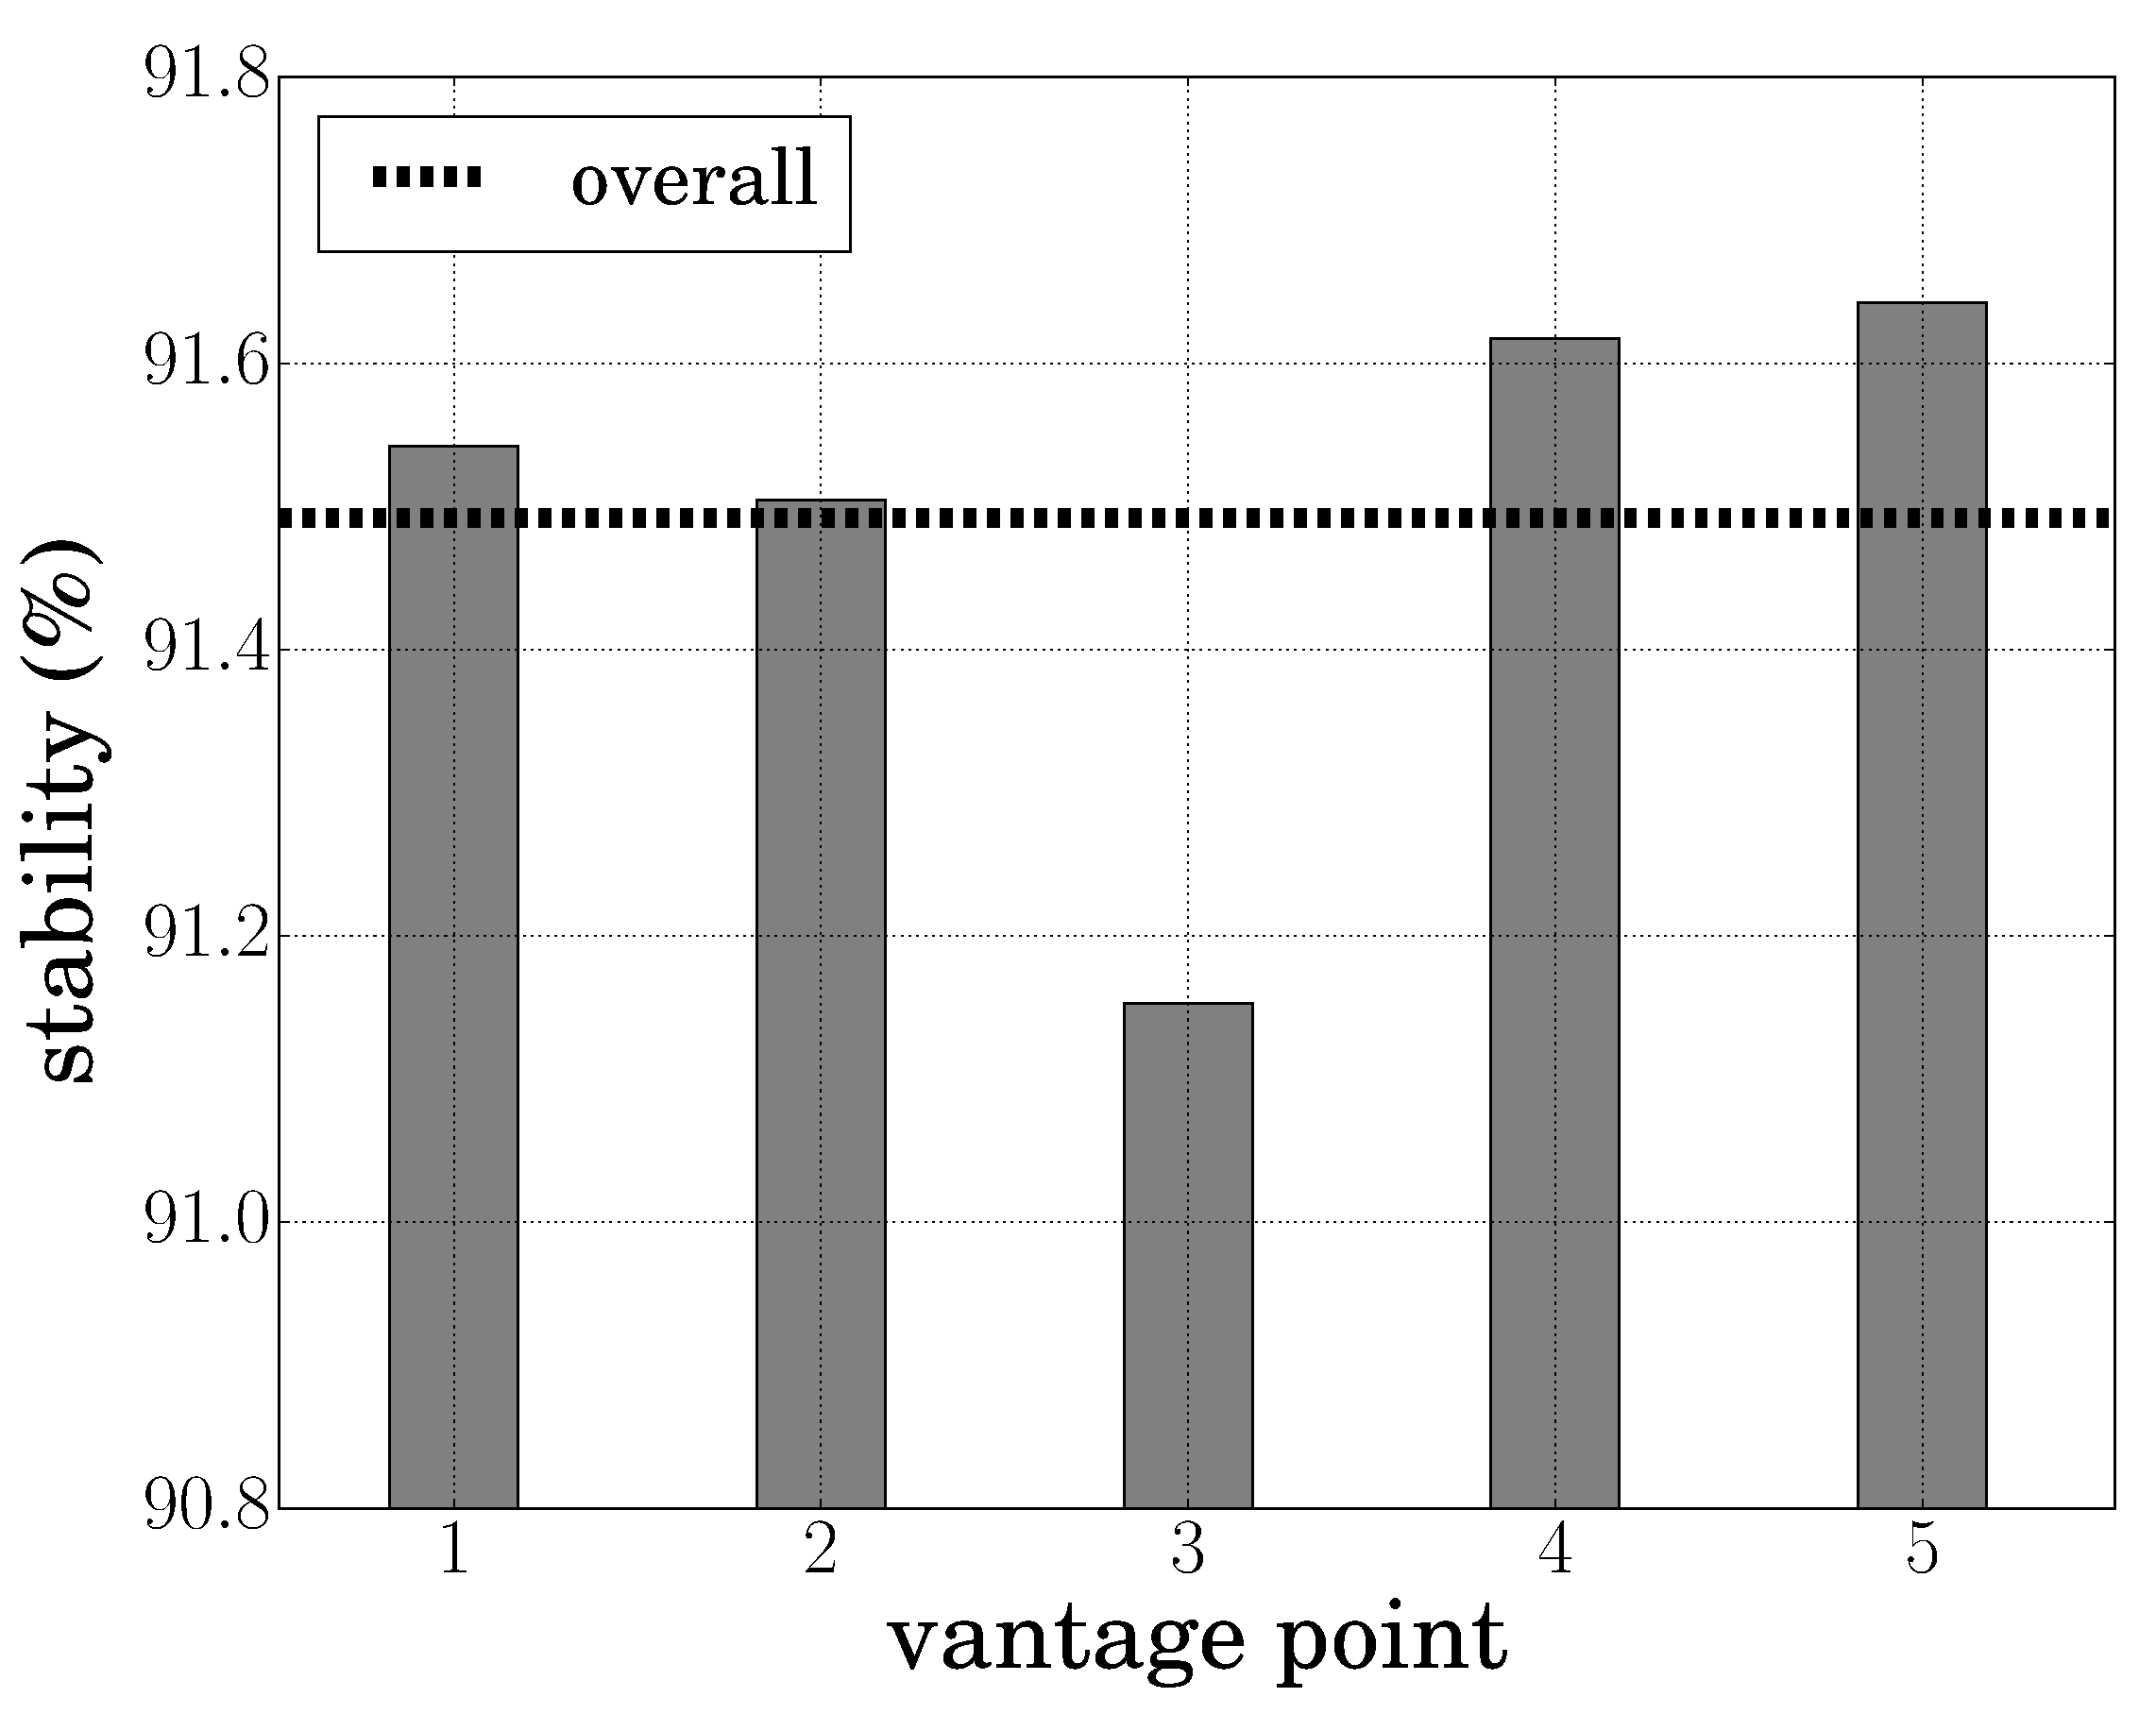
\includegraphics[width=0.7\textwidth]{Pics/Percentage_stability_5VP_time.eps}
	\caption{Overall percentage of stability observed at five different VPs.}
	\label{fig:Percentage_stability_5VP_time}
\end{figure}
%-< END FIGURE >-----------------------------------------------------------------

%-< FIGURE >--------------------------------------------------------------------
\begin{figure}[t]
	\centering
	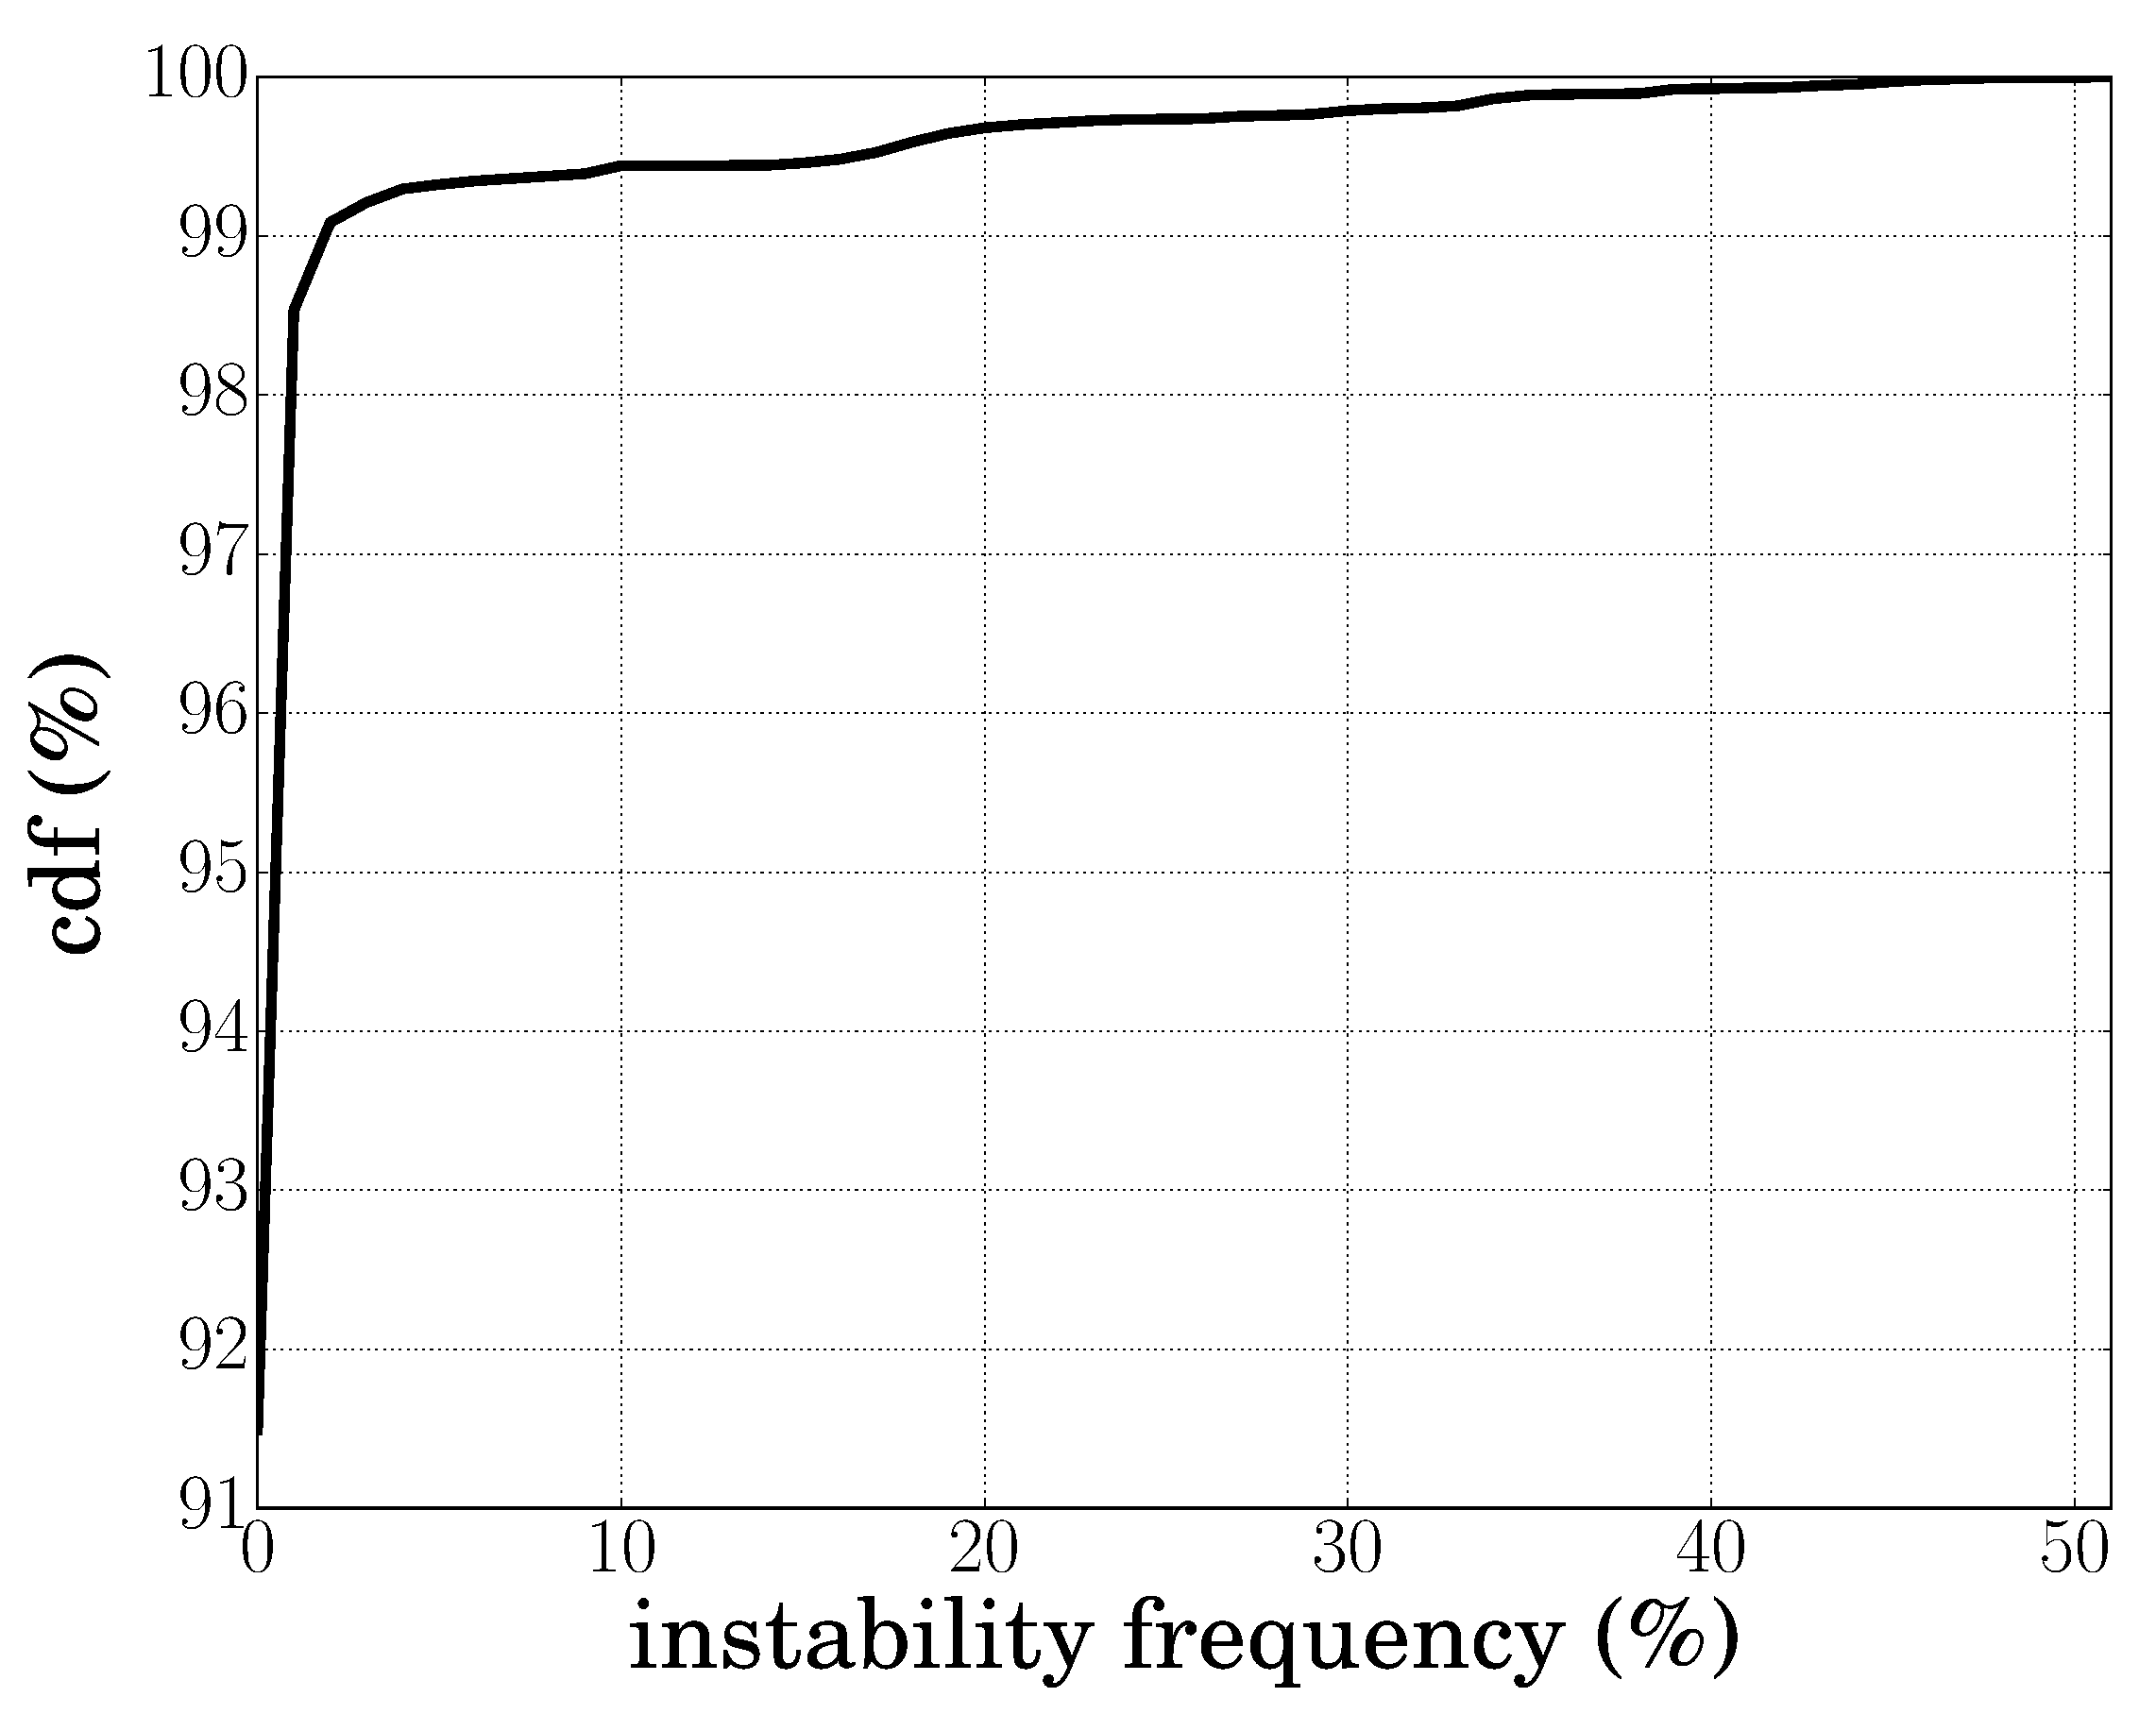
\includegraphics[width=0.7\textwidth]{Pics/cdf_instability_occur.eps}
	\caption{CDF of instability frequency. X-axis is instability frequency, indicating the ratio of instability occurrence number for one <$EID, MR, VP$> tuple over total experiment number.}
	\label{fig:cdf_instability_occur}
\end{figure}
%-< END FIGURE >-----------------------------------------------------------------


%-< FIGURE >--------------------------------------------------------------------
\begin{figure}[t]
	\centering
    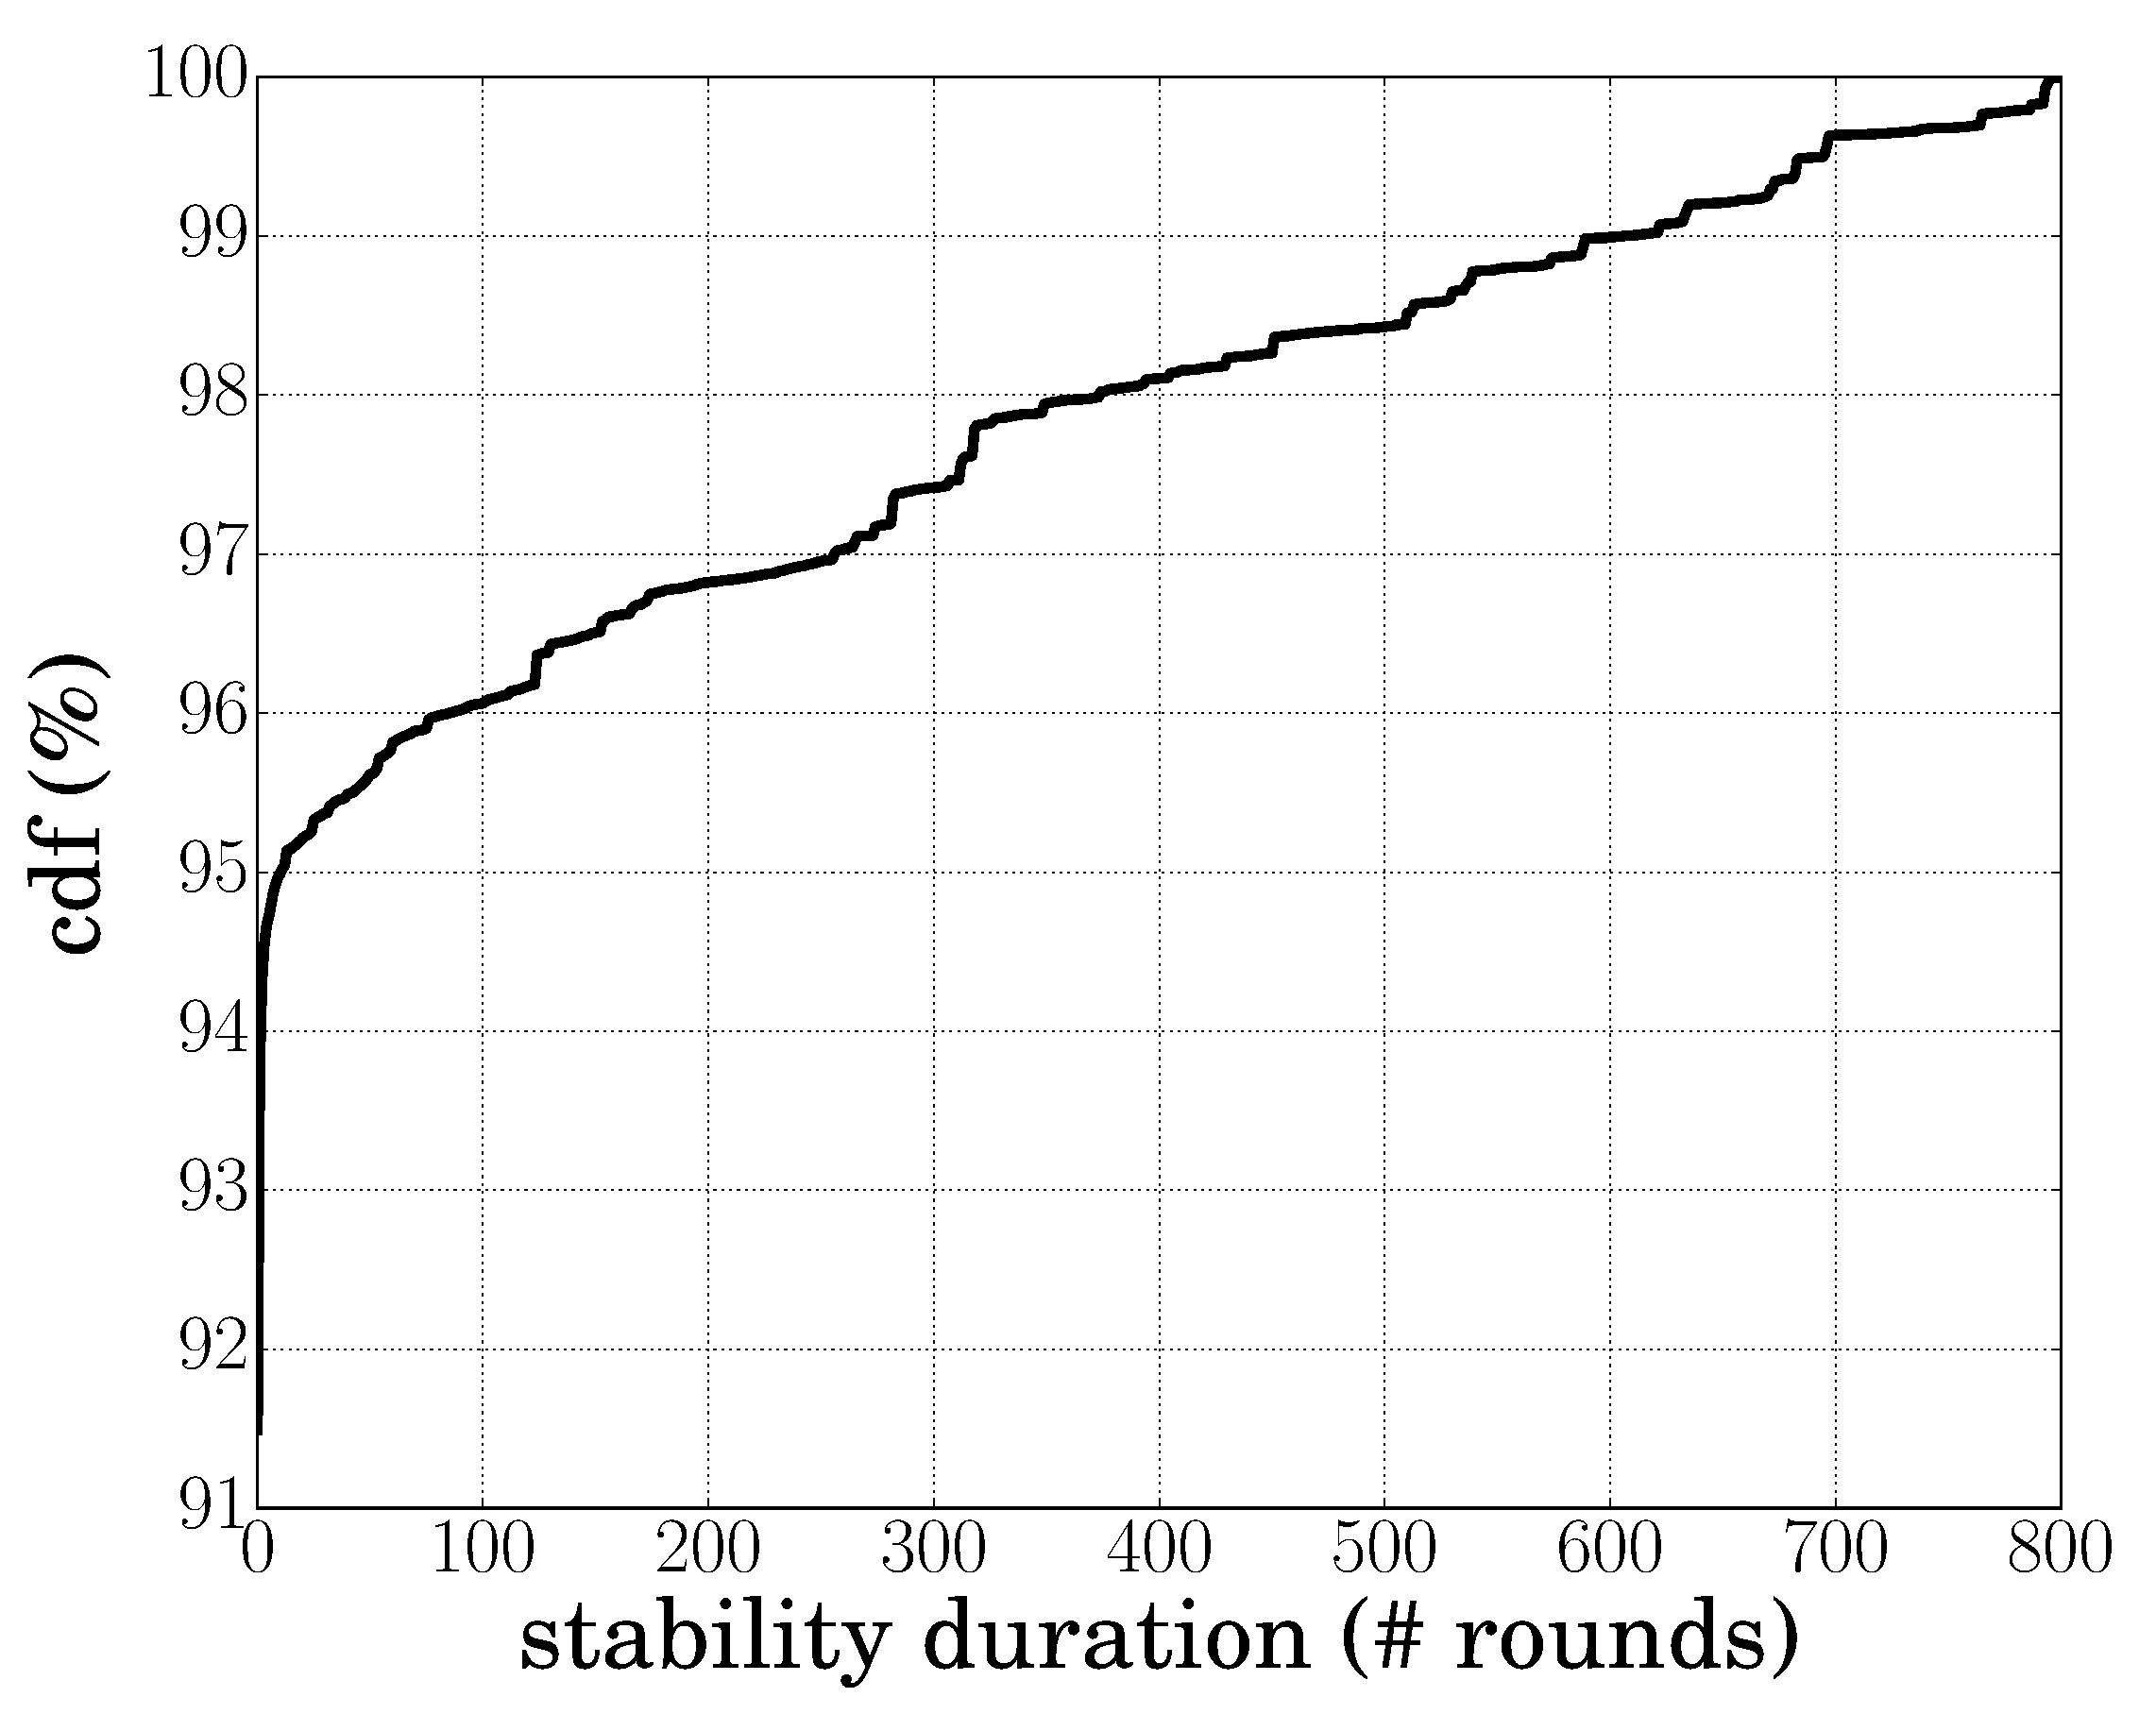
\includegraphics[width=0.7\textwidth]{Pics/cdf_stability_duration.eps}
	\caption{CDF of stability duration (in number of experimental rounds). X-axis is stability duration, indicating during how many experiment rounds that the mapping for one <$EID, MR, VP$> tuple is stable.}
	\label{fig:cdf_stability_duration}
\end{figure}
%-< END FIGURE >-----------------------------------------------------------------

Fig.~\ref{fig:cdf_instability_occur} complements Fig.~\ref{fig:Percentage_stability_5VP_time} by showing, for each tuple <$EID, MR, VP$>, the frequency $f_{<EID, MR, VP>}$ at which mappings are different, by using the following definition: 
\begin{equation}
f_{<EID, MR, VP>} = \frac{\text{\# Instabilities}}{\text{\# Experiments}}\times100\%.
\end{equation}
Thus, if the instability frequency $f_{<EID, MR, VP>}$ is 0\%, it means that such a tuple is always stable during the whole experiment, i.e., its Map-Replies are always the same. On the contrary, a tuple <$EID, MR, VP$> with instability frequency of 100\% indicates that its current Map-Reply is never identical to the previous ones, i.e., its Map-Replies change at every experiment round.

Fig.~\ref{fig:cdf_instability_occur} shows the CDF of the mapping change frequency (i.e., instability frequency). It shows the probability where the instability frequency equals to zero is 91.49\%, which is coherent with the result in Fig.~\ref{fig:Percentage_stability_5VP_time} (dashed line) and means that the mapping is globally stable. Apart from the stability case, the others ($100.0\%-91.49\%$) belong to the mapping changes case, i.e., instability. This CDF also shows when the instability frequency equals to 1\%, the CDF reaches to 98.53\%, which indicates that among the instability cases, 82.77\% ($\frac{98.53-91.49}{100.0-91.49}\%$) of all mapping changes events have an instability frequency less than 1\%. We can deduce that mapping changes, if they occur, are rare events. The existence of instability frequency around 50\% means that, in some cases, even though it is rather rare, the mapping changes occurs almost one time every two experiment rounds.

While Fig.~\ref{fig:cdf_instability_occur} indicates that mappings can potentially change frequently, Fig.~\ref{fig:cdf_stability_duration} shows the CDF of the stability duration, i.e., for how many experiment rounds a mapping remains stable. We observe that the majority of instabilities has a stability duration of 1 experiment round. This fact shows that the mapping change occurs during a measurement period (i.e., 30 minutes, the interval between two experiment rounds). At the other side of the curve, stability lasts up to 800 experiment rounds are observed, indicating that the mapping changed at the very beginning of or the end of the measurements we performed. In the dataset we identified both cases. To further understand the instability, we classify it into four categories:
\begin{itemize}
  \item \emph{New Deployment}: the Map-Replies of a tuple <$EID, MR, VP$> mix two different types: Negative Map-Reply and LISP Map-Reply. %It is caused more often by turning on/off the xTRs than the real deployment of LISP sites. 
  % It is caused more often by changing the configurations of the xTRs between using LISP and not than the real deployment of LISP sites. 
  Since the changes between the different types of Map-Reply are mainly caused by the deployments of new LISP-Sites, we make this case named New Deployment.
  \item \emph{Statistical outliers}: the Map-Replies of a tuple <$EID, MR, VP$> change more frequently than usually seen. In our measurements, outliers correspond to mappings that change at least 3 times during a day.    
  \item \emph{Mobility}: the Map-Replies of a tuple <$EID, MR, VP$> are explicitly tagged with the mobility bit as specified in RFC6830~\cite{rfc6830}.  
  \item \emph{Reconfiguration}: all cases that fit neither into the New Deployment case nor the Statistical outliers case.
\end{itemize}

%-< TABLE >--------------------------------------------------------------------
\begin{table}[!tb]
	\centering
	\caption{Percentage of Instabilities by Category}
	\label{tab:Proporition_instability}{
	\resizebox{0.7\textwidth}{!}{%
		\begin{tabular}{@{}c|c|c|c@{}}
			\hline\hline
			New Deployment  &Statistical outliers&  Mobility &  Reconfiguration \\ \hline
			72.36\%  &7.23\%&  0\%  &  20.41\%     	\\ \hline \hline                 
		\end{tabular}
	}}
\end{table}
%-< END TABLE >--------------------------------------------------------------------

Tab.~\ref{tab:Proporition_instability} presents the percentage of observations for the four categories. New Deployments dominate the total unstable cases with a percentage of 72.36\%, followed by Reconfiguration with 20.41\%, and Statistical outliers with 7.23\%. Throughout the dataset, we did not observe any Mobility event, probably because the mobility specifications were not yet implemented at the time of measurements. Therefore, we omit the Mobility category in the rest of this chapter.

New Deployments are the most common instabilities and we used spectral analysis with Fourier transforms and auto-correlation to understand if such events are correlated between themselves. This analysis shows that New Deployments are equally spread over the whole measurement period, i.e., their occurrence per day is relatively constant. We performed the same study on the Reconfiguration category and Statistical outliers and reached the same conclusion, i.e., the absence of correlations between events.

Since New Deployments are incidental events that can happen at any time, no particular duration is observed for this category of instabilities. Moreover, as New Deployments account for 72.36\% of instabilities, it significantly impacts the duration distributions shown in Fig.~\ref{fig:cdf_stability_duration}, explaining the relatively smooth evolution of the CDF. On the contrary, Statistical outliers are characterized by very frequent changes and they bias the distribution around the lowest duration values, explaining the relatively high number of observations for small duration.

%-< FIGURE >--------------------------------------------------------------------
\begin{figure}[!t]
	\centering
	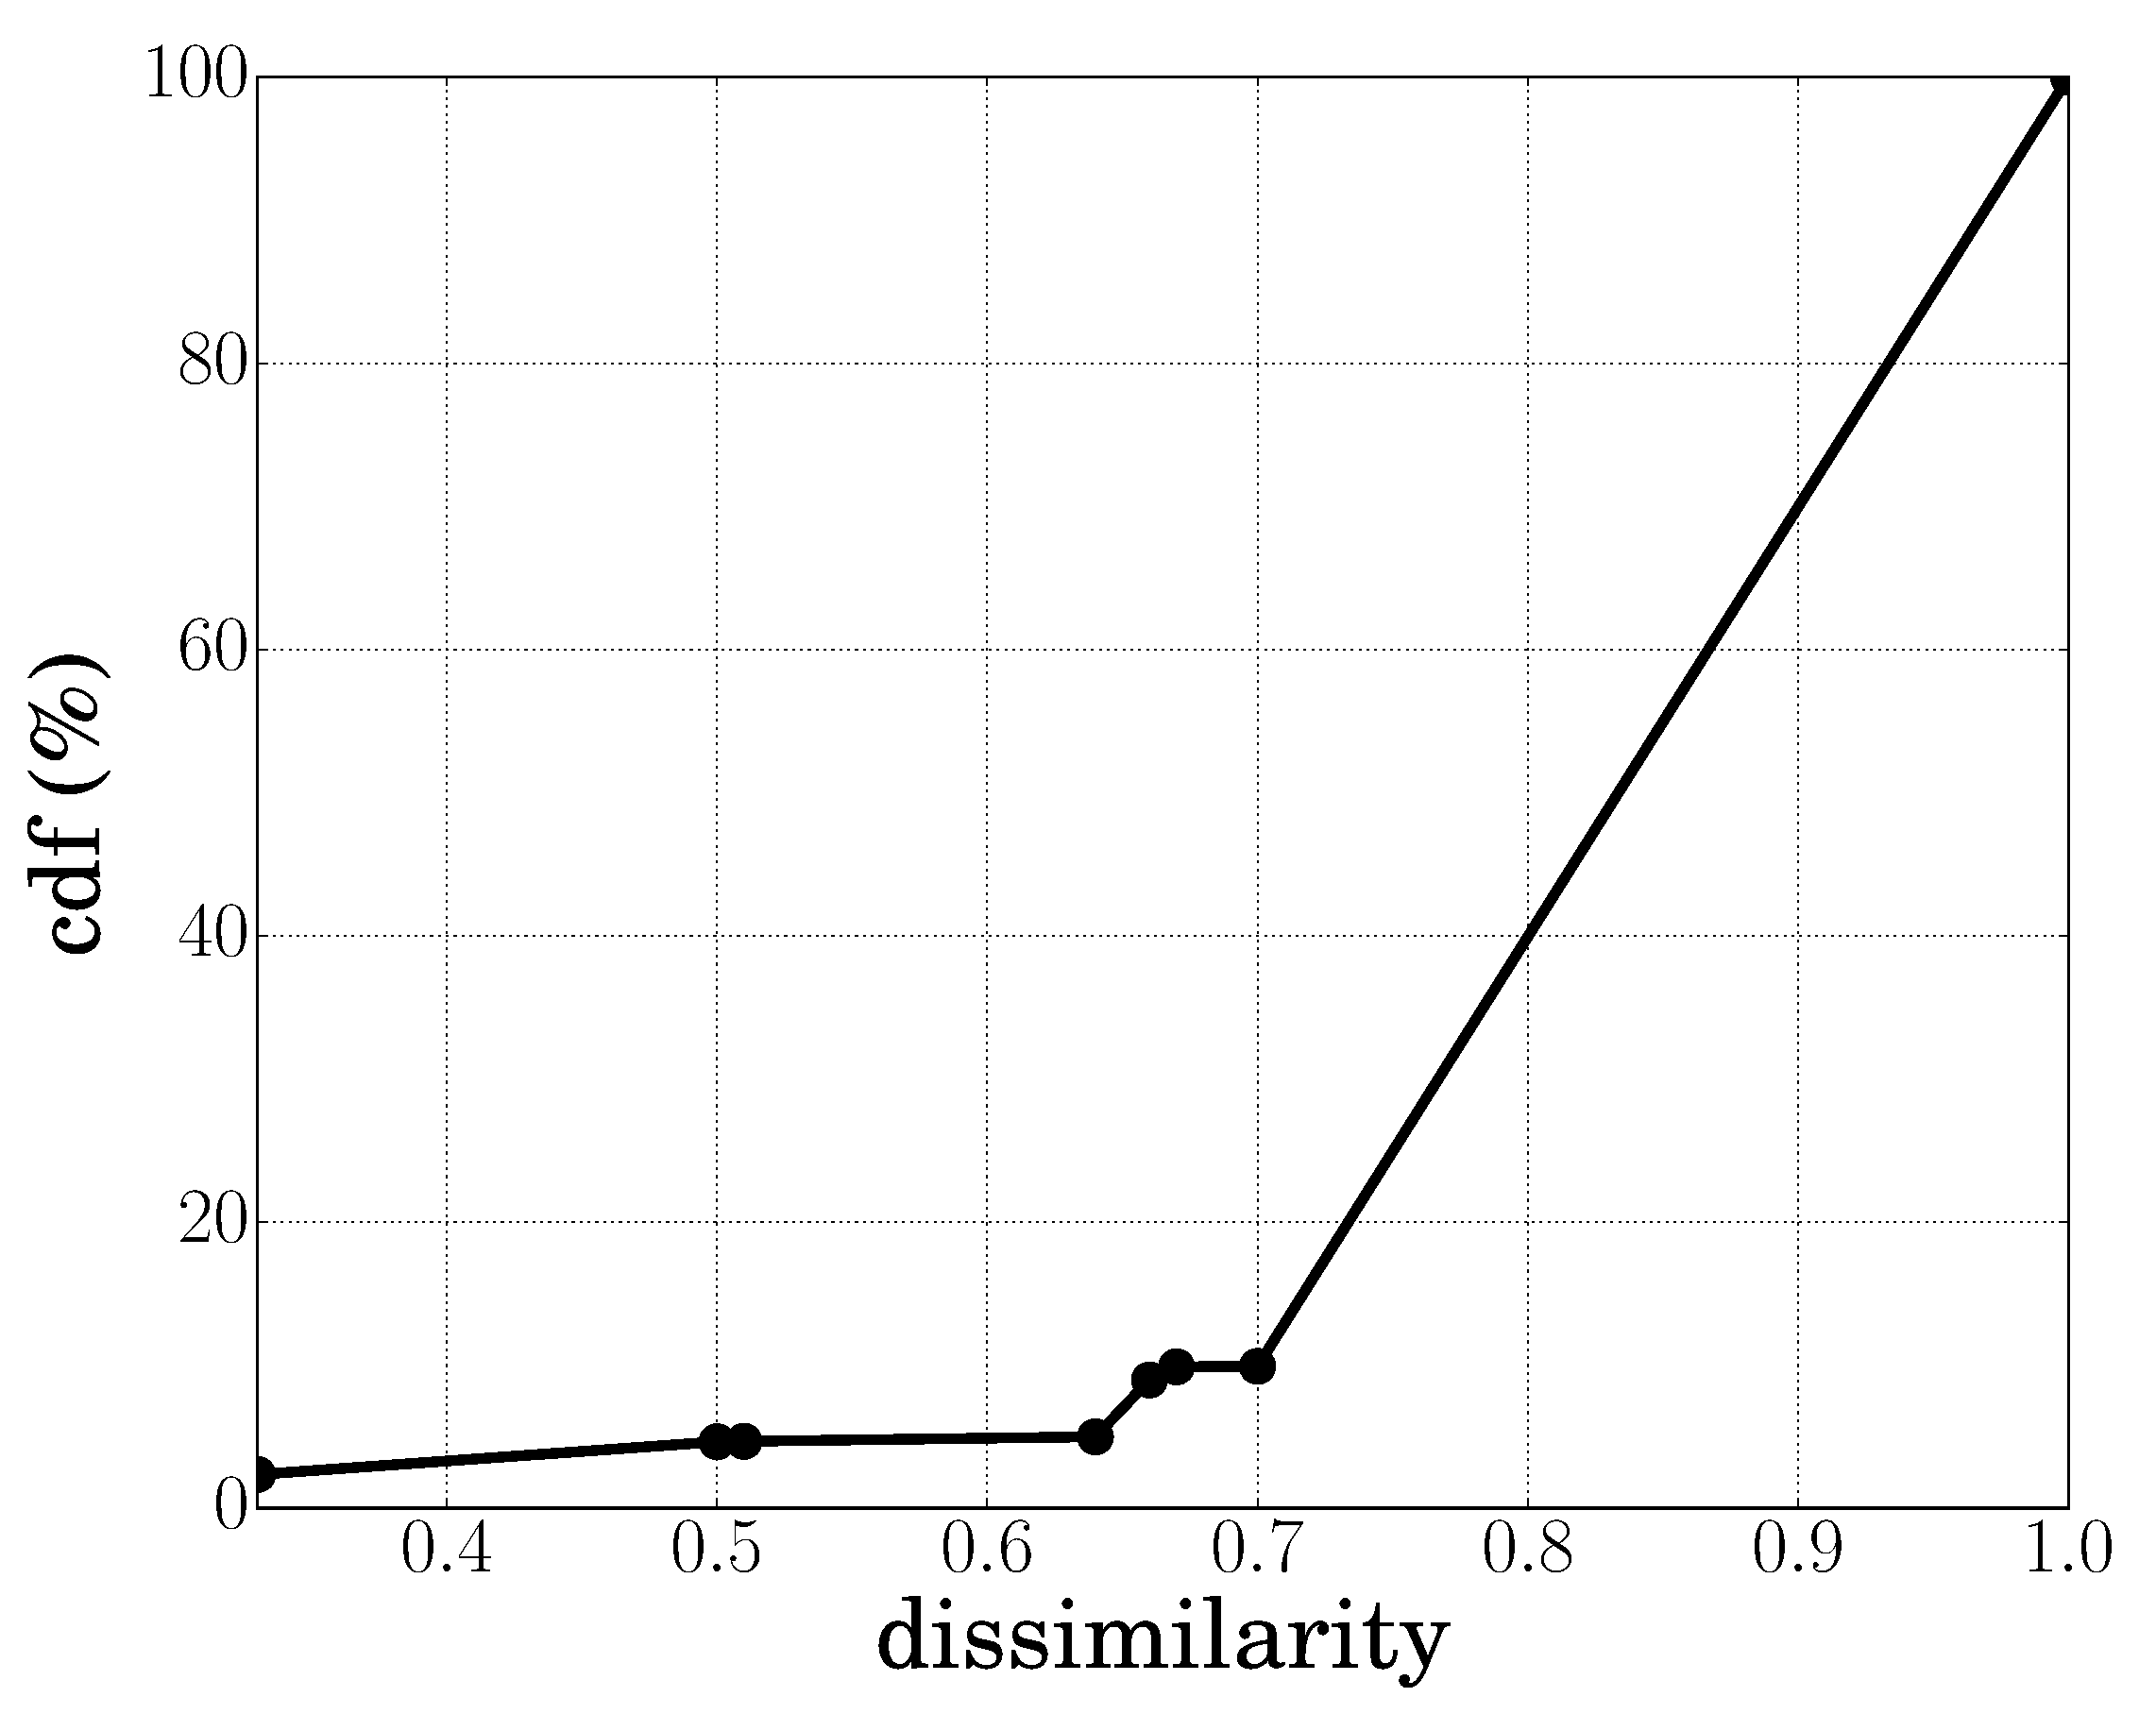
\includegraphics[width=0.7\textwidth]{Pics/cdf_dissmilarity.eps}
	\caption{CDF of the dissimilarity among different types of instabilities.}
	\label{fig:cdf_dissmilarity}
\end{figure}
%-< END FIGURE >-----------------------------------------------------------------

To characterize the mapping changes happening during instabilities, we derived the following \emph{dissimilarity} metric $d(m_i,m_j) = 1 - \frac{ \left|m_i \cap m_j\right|}{\left|m_i \cup m_j\right|}$, based on the Jaccard similarity coefficient, where $m_x$ is the RLOC set of mapping $x$. A dissimilarity of 1 indicates that no RLOCs are shared between the two compared mappings, while a dissimilarity of 0 indicates that the RLOC sets are the same. Fig.~\ref{fig:cdf_dissmilarity} shows the CDF of the mappings' dissimilarity for each unstable <$EID, MR, VP$> tuple. In our experiment, the dissimilarity results are discrete (as the discrete points shown in the Fig.~\ref{fig:cdf_dissmilarity}) in a range from 0.33 to 1.0. As one can expect, the most likely dissimilarity is 1 in 90.09\% of the total number of instabilities. These observations mostly come from New deployment case where before turning on the xTR, no RLOC is provided with the Negative Map-Reply (RLOC set is empty), hence, switch to a LISP Map-Reply implies a full change in the RLOC set. As 90.09\% is larger than the 72.36\% of New deployments share, it indicates as well that complete change of the RLOC set have also been observed during Reconfiguration and Statistical outliers. For the rest, no particular trend can be observed showing that changes of RLOC set can actually take any form.


%-< SECTION >--------------------------------------------------------------------
\section{Mapping system consistency evaluation}
\label{sec:mds_consistency}
% In this section, we discuss the consistency of the mapping system respectively by MR and by VP.

In this section, we discuss the consistency of the mapping system respectively by MR and by VP. More precisely, we consider that a tuple of <$EID, *, VP$> exhibits consistency, if all the Map-Replies from different MRs, for a certain EID, observed at a given VP are identical at the same time (same experiment round). This kind of consistency is denoted as \emph{consistency by MR}. Similarly, if all the Map-Replies sent by a specific MR, for a certain EID, and observed at different VPs are identical at every experiment round, then we consider that a tuple of <$EID, MR, * $> is consistent, and denote it as \emph{consistency by VP}. Otherwise, for cases not falling in the above two, we simply say that there exists \emph{inconsistency}. 

Overall, throughout the whole dataset, we found that 86.3\% of observations of all <$EID, *, VP$> tuples are consistent, which indicates that non-identical Map-Replies from different MRs are uncommon. Similarly, consistency by VP is observed in 90.48\% of observations of all <$EID, MR, * $> tuples, showing that the Map-Replies received at different VPs are usually identical. In the following, Sec.~\ref{subsec:mds_consistency_MR} will go deeper in the analysis of consistency by MR, proposing as well several types of inconsistency; then Sec.~\ref{subsec:mds_consistency_VP} will provide thorough analysis of consistency by VP.


%-< SUB SECTION >--------------------------------------------------------------------
\subsection{Consistency evaluation by MR}
\label{subsec:mds_consistency_MR}
% \begin{itemize}[noitemsep,topsep=0pt]
%     \item The overall percentage of consistency by MR is 86.3\%.
%     \item CDF of the inconsistency frequency by MR.
%     \item For the inconsistency by MR, we classify into 2 cases:
%     \begin{itemize}[noitemsep,topsep=0pt]
%         \item Map-Reply Type: is around 98.34\%.
%         \item RLOC set: 1.66\%.
%     \end{itemize}
% \end{itemize}

The overall percentage of consistency by MR is 86.3\% (see the dashed line on Fig.~\ref{fig:Percentage_consistency_5VP_MR}), meaning that across the whole experiment the inconsistency among the Map-Replies sent by different MRs is not common. Yet, we can also observe from Fig.~\ref{fig:Percentage_consistency_5VP_MR} that different VPs show some deviations from the overall consistency by MR, reflecting the fact that while certain VPs receive the same Map-Reply from different MRs, some other VPs receive inconsistent responses. Such deviation is very small (no more than 2.77\%) among different vantage points, indicating that it remains a relatively rare event. These results show that the mapping system is consistent among different MRs in general, but the inconsistency exists at the same time with a percentage around 13.7\%.  In the following of this section, we go deeper in this issue, exploring the reasons why the few observations exhibit
inconsistency by MR.

%-< FIGURE >--------------------------------------------------------------------
\begin{figure}[!t]
	\centering
	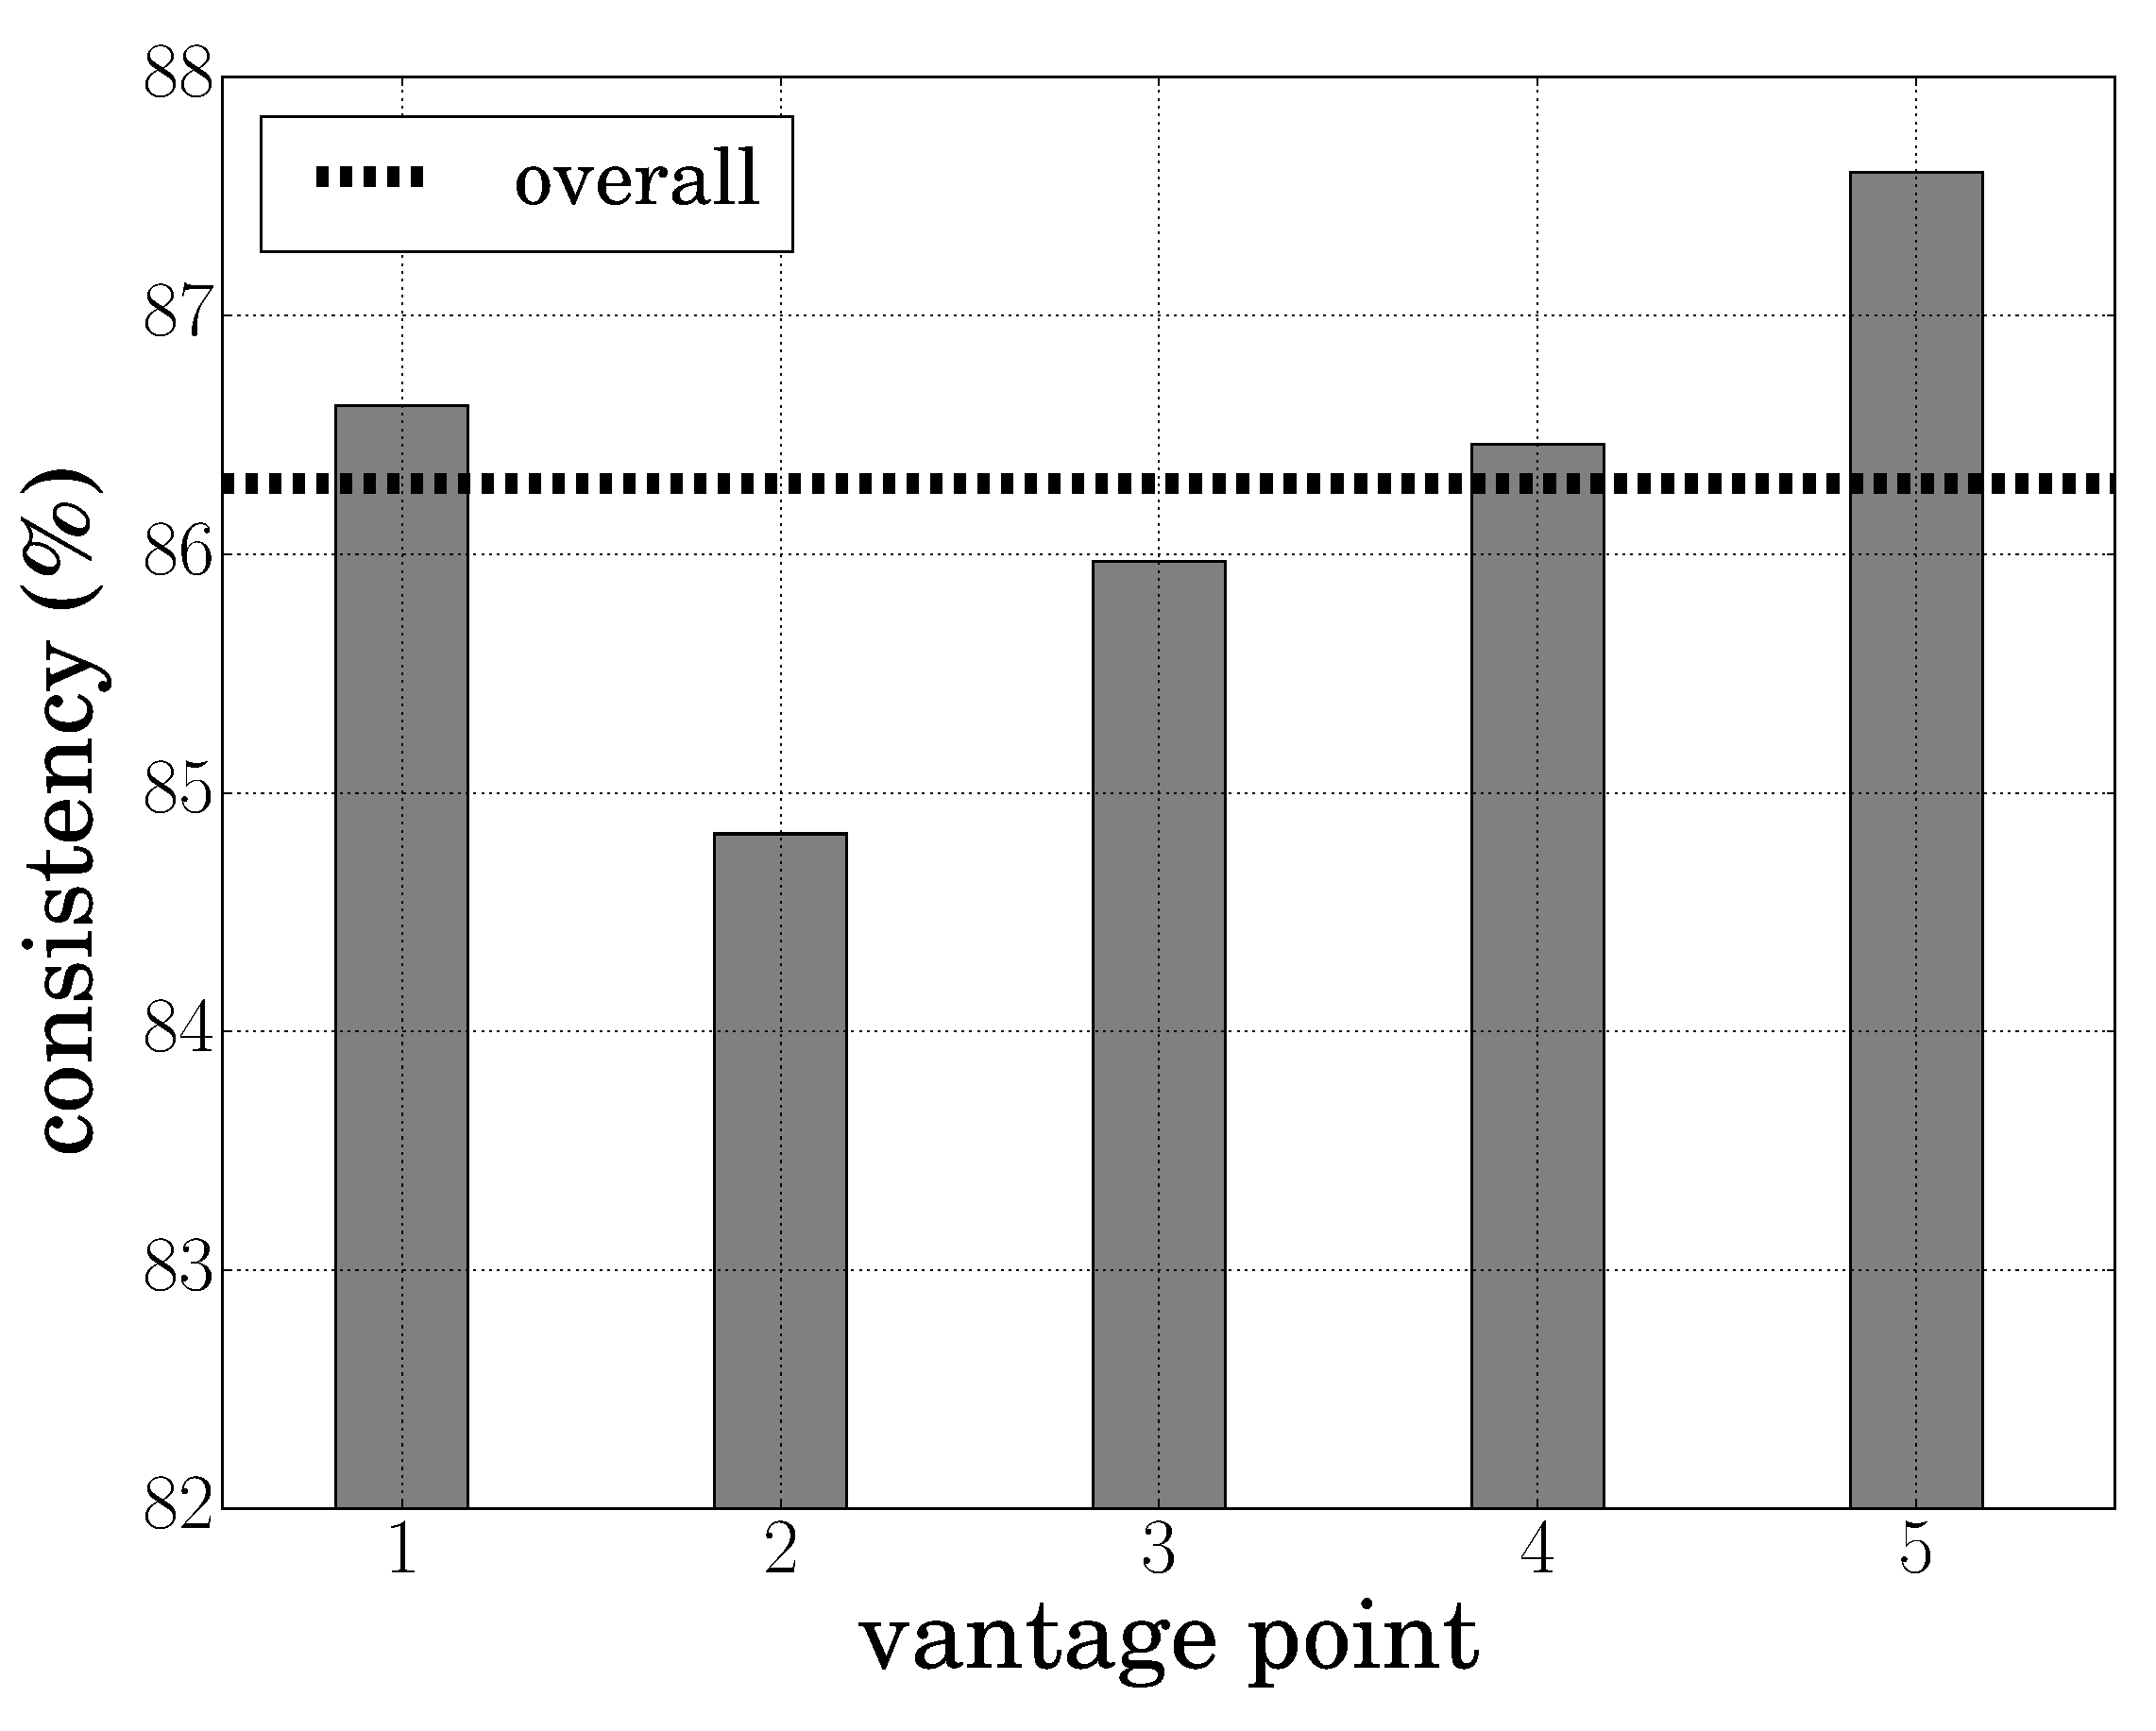
\includegraphics[width=0.7\textwidth]{Pics/Percentage_consistency_5VP_MR.eps}
	\caption{Overall consistency by MR at 5 different Vantage Points.}
	\label{fig:Percentage_consistency_5VP_MR}
\end{figure}
%-< END FIGURE >--------------------------------------------------------------------

We compute the CDF of the inconsistency frequency by MR: $f_{<EID, *, VP>}$, i.e.,  the probability of inconsistency frequency over all <$EID, *, VP$> tuples, by using the following definition: 
\begin{equation}
f_{<EID, *, VP>}= \frac{\text{\# Inconsistencies by MR}}{\text{\# Experiments}}\times100\%.
\end{equation}
For a <$EID, *, VP$> tuple, an inconsistency frequency of 0\% means that all Map-Replies from all of the different MRs for one EID are the same at each experiment round throughout the whole measurement campaign.  For a <$EID, *, VP$> tuple, an inconsistency frequency of 100\% means that at each experiment round during the whole measurement campaign, there is at least one MR replying a Map-Reply different from the replied by other MRs. The resulting CDF of inconsistency frequency is shown on Fig.~\ref{fig:cdf_incons_occur_MR}. The value 0\% of inconsistency frequency has a probability of 82.38\%, indicating that through all the dataset, there are 82.38\% of <$EID, *, VP$> tuples that are always consistent by MR at whichever VP. Yet, it is worth noticing that this value is lower than the overall consistency of 86.3\% shown in Fig.~\ref{fig:Percentage_consistency_5VP_MR}. The reason of such difference lays in the fact that, when we analyze the 0\% inconsistency frequency, we just take into account those common EIDs exhibiting a consistency by MR in all VPs. Hence, 82.38\% represents the subset of the EIDs considered in the former percentage and is the lower bound, guaranteeing that 82.38\% of <$EID, *, VP$> tuples always have consistent responses, regardless of the VP. In addition, the inconsistency frequency concentrates at a very low range, since a sharp increase occurs between 0\% and 2\% with a growth of 16.15\%. % (98.53\% - 82.38\%). 
It indicates that the <$EID, *, VP$> tuples classed as inconsistent do actually receive inconsistent responses rarely, hence, demonstrating that the mapping system is generally consistent. Yet, in very few cases (only 0.5\%), the inconsistency between different MRs occurs all the time.

%-< FIGURE >--------------------------------------------------------------------
\begin{figure}[!t] 
	\centering
	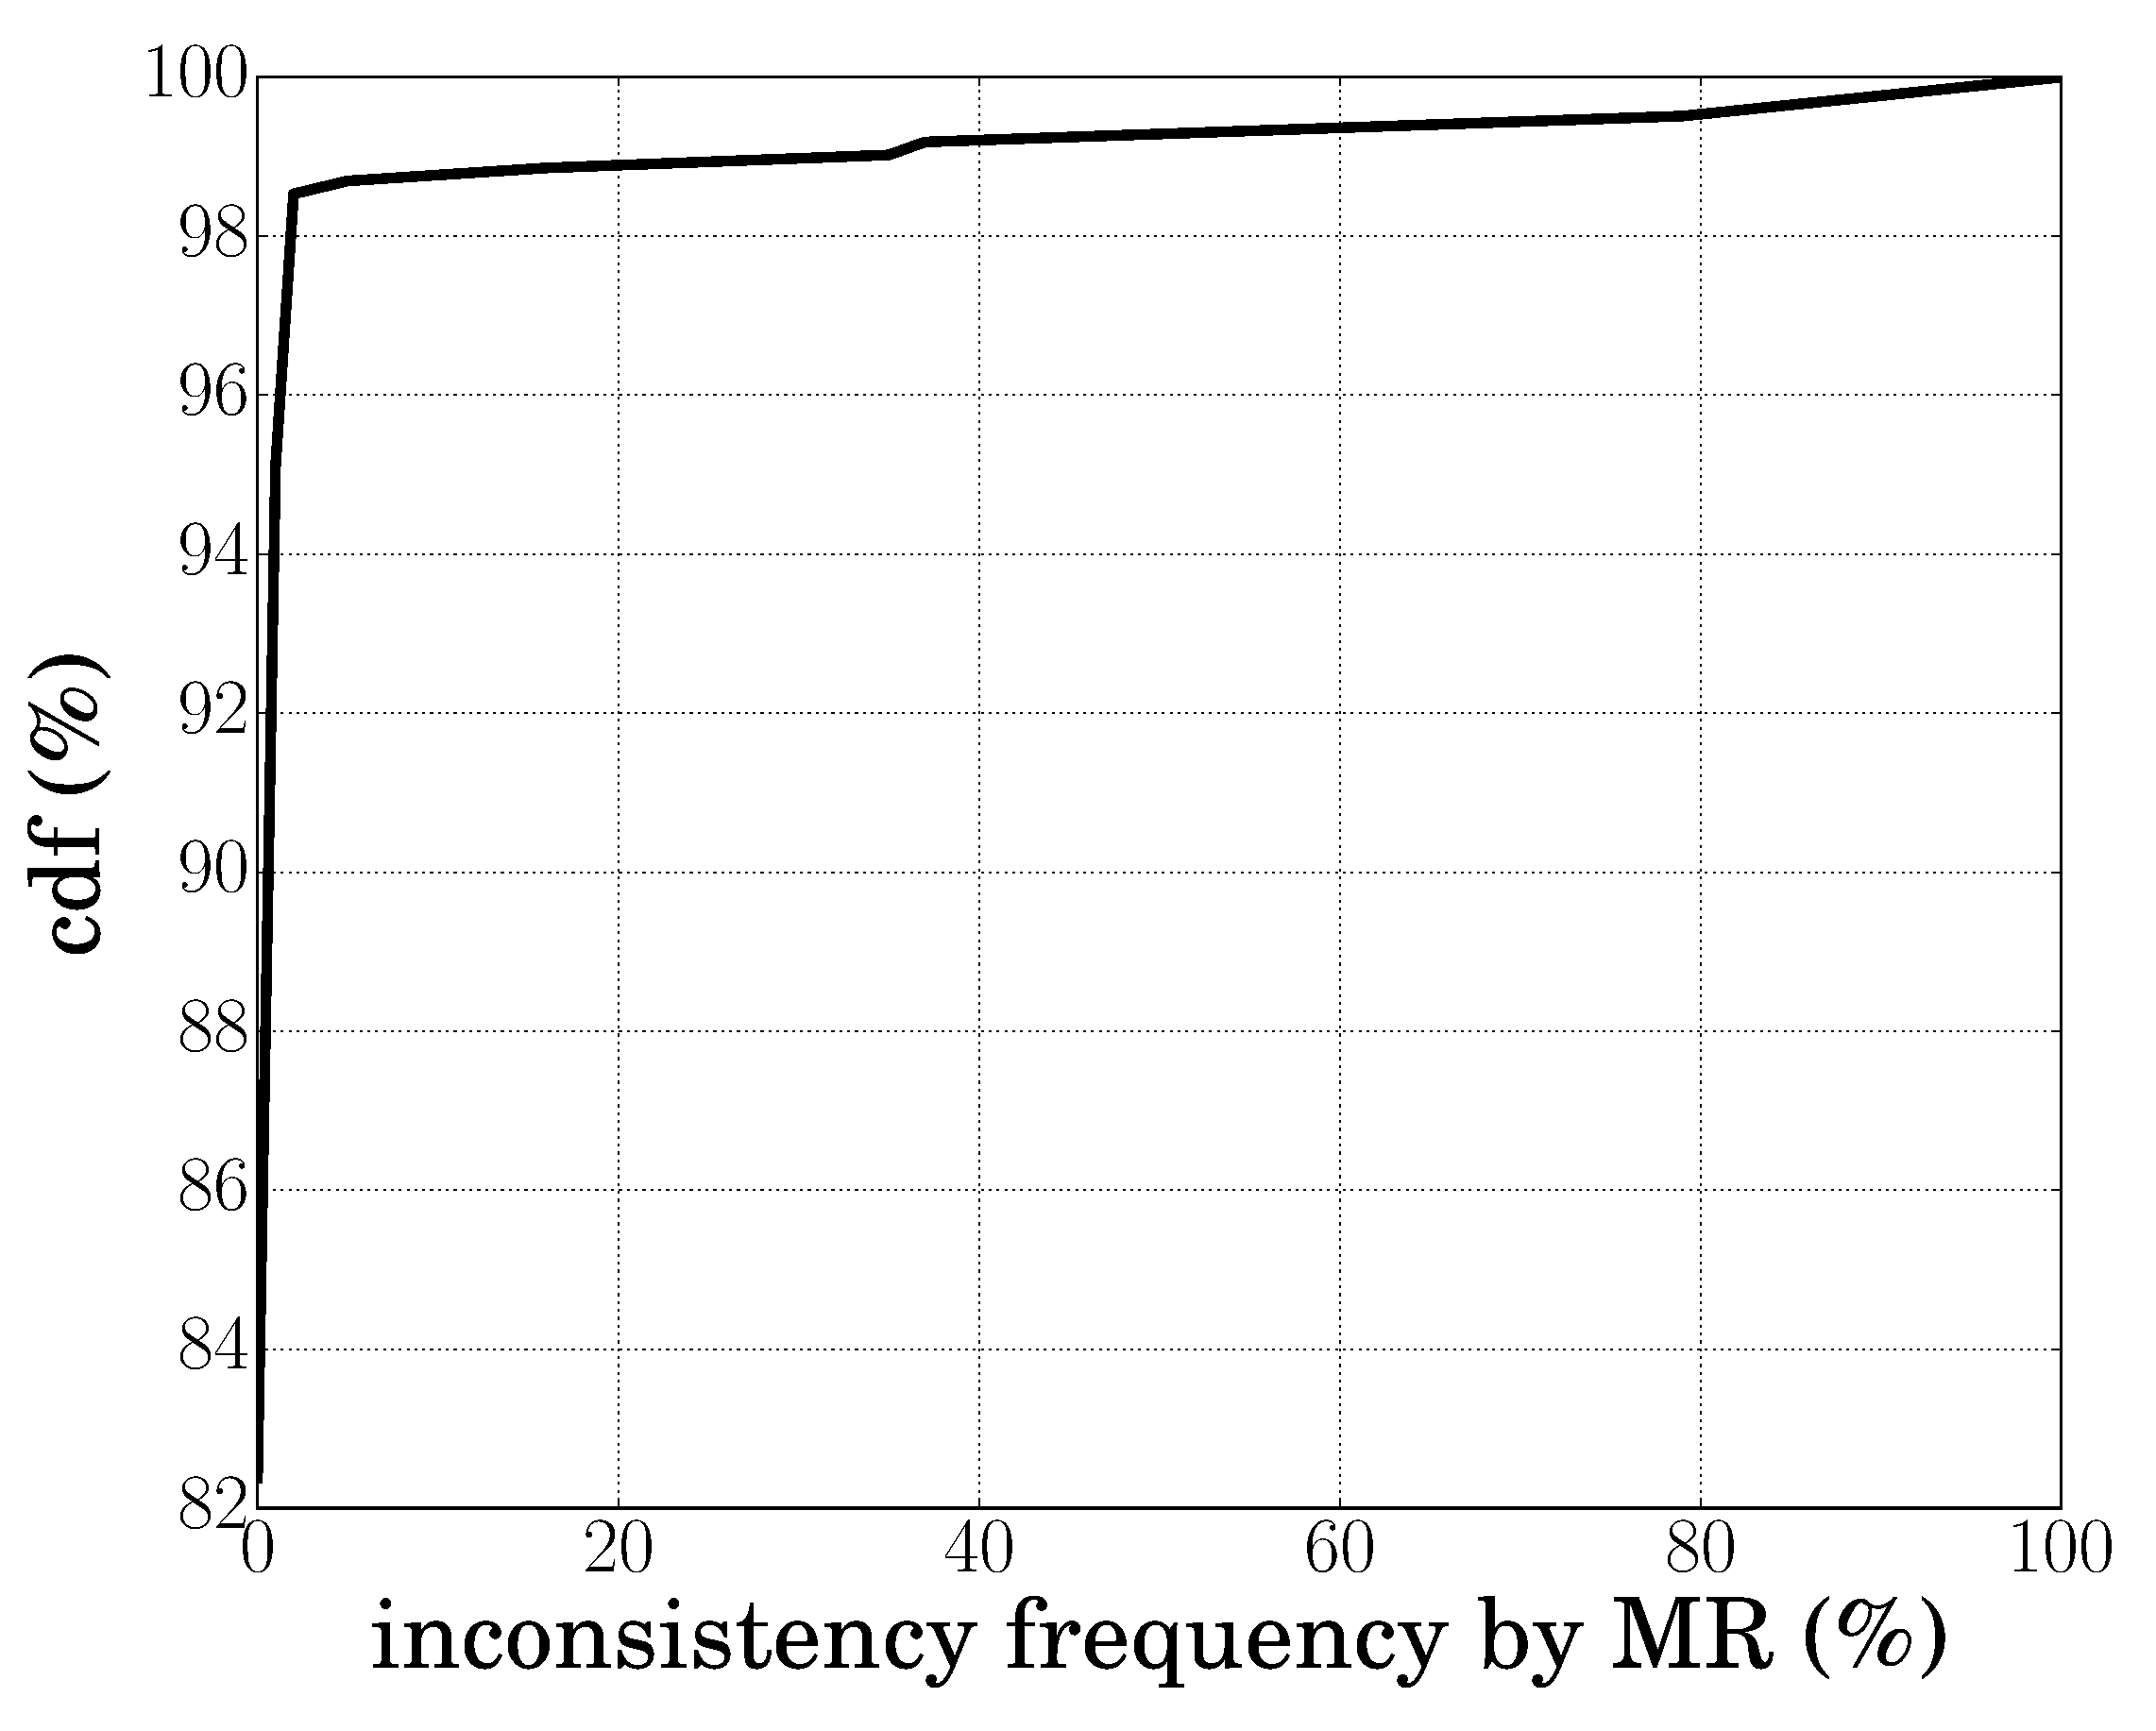
\includegraphics[width=0.7\textwidth]{Pics/cdf_incons_occur_MR.eps}
	\caption{Cumulative Distribution Function of inconsistency frequency by MR. X-axis is inconsistency frequency by VP, indicating the ratio of inconsistency occurrence for each <$EID, *, VP$> tuple over total experiment number.}
	\label{fig:cdf_incons_occur_MR}
\end{figure}
%-< END FIGURE >--------------------------------------------------------------------

So far, the analysis indicates that the mapping system is consistent by MR in general, but the inconsistency indeed exists. To have a closer look to the inconsistency, we further cluster it into two cases:
\begin{itemize}[noitemsep,topsep=0pt]

\item \textbf{Map-Reply Type}:, The type of Map-Reply provided by the 13 MRs for a specific <$EID, *, VP$> tuple is different, meaning that some MRs provide LISP Map-Reply while others return a Negative Map-Reply. The difference of received Map-Reply type leads the xTRs to use a different way to send the packets, i.e., xTRs receiving a LISP Map-Reply sends LISP-encapsulated packets by using the obtained RLOCs, while xTRs receiving a Negative Map-Reply will forward the conventional packets (i.e., without LISP-encapsulation).
\item \textbf{RLOC set}: All the Map-Replies returned by the 13 MRs for a <$EID, *, VP$> tuple belong to LISP Map-Reply type, but the associated attributes (cf.  Tab.~\ref{tab:List_of_possible_changes} from Sec.~\ref{sec:mds_methodology}) are different.  For instance, some Map-Replies may contain RLOC$_1$, while some others convey RLOC$_2$ (i.e., the RLOC address is not identical); or some Map-Replies have only one RLOC, whereas others have multiple RLOCs (i.e., the RLOC number is different), and so on. The difference in such Map-Replies could lead the requesting xTRs to select different destination RLOCs. 
\end{itemize}

The large majority of inconsistencies, around 98.34\%, are Map-Reply Type, probably because there is an update of mapping information in the mapping system for the New Deployment case. Not all of the 13 MRs simultaneously update the mapping information, meaning that a convergence time is needed so that the global mapping information maintained in all parts of the mapping system is synchronized. If VPs query the mapping system during this convergence period, some MRs will still provide Negative Map-Replies, while other (already updated) MRs will forward the Map-Requests towards the corresponding ETRs, which in turn will send the updated LISP Map-Replies, and vice versa. This situation contributes to the inconsistency frequency around 1\%, which means that there is only once or twice inconsistency between Map-Replies from different MRs for one specific EID, since changing the status of xTR is not frequent.

Just few inconsistencies, only 1.66\%, are caused by the RLOC set. This scenario usually occurs for those EIDs whose RLOCs change frequently over time (the case of Statistical outliers instability). So, because of the convergence time of the mapping system, it is very difficult to guarantee that every MR can provide the same LISP Map-Reply at every experiment round. This reason for changes in the RLOC set is most probably due to traffic engineering policies. Similarly as the previous case, when different MRs provide a different RLOC set for a specific EID, the requesting xTRs may end up using different RLOCs to reach the same destination EID.
 

%-< SUB SECTION >--------------------------------------------------------------------
\subsection{Consistency evaluation by VP}
\label{subsec:mds_consistency_VP}
% \begin{itemize}[noitemsep,topsep=0pt]
%     \item The overall percentage of consistency by VP is 90.48\%.
%     \item CDF of the inconsistency frequency by VP.
%     \item For the inconsistency by MR, we classify into 2 cases:
%     \begin{itemize}[noitemsep,topsep=0pt]
%         \item Map-Reply Type: is around 89.06\%.
%         \item RLOC set: 10.94\%.
%     \end{itemize}
% \end{itemize}

%-< FIGURE >--------------------------------------------------------------------
\begin{figure}[!t]
	\centering
	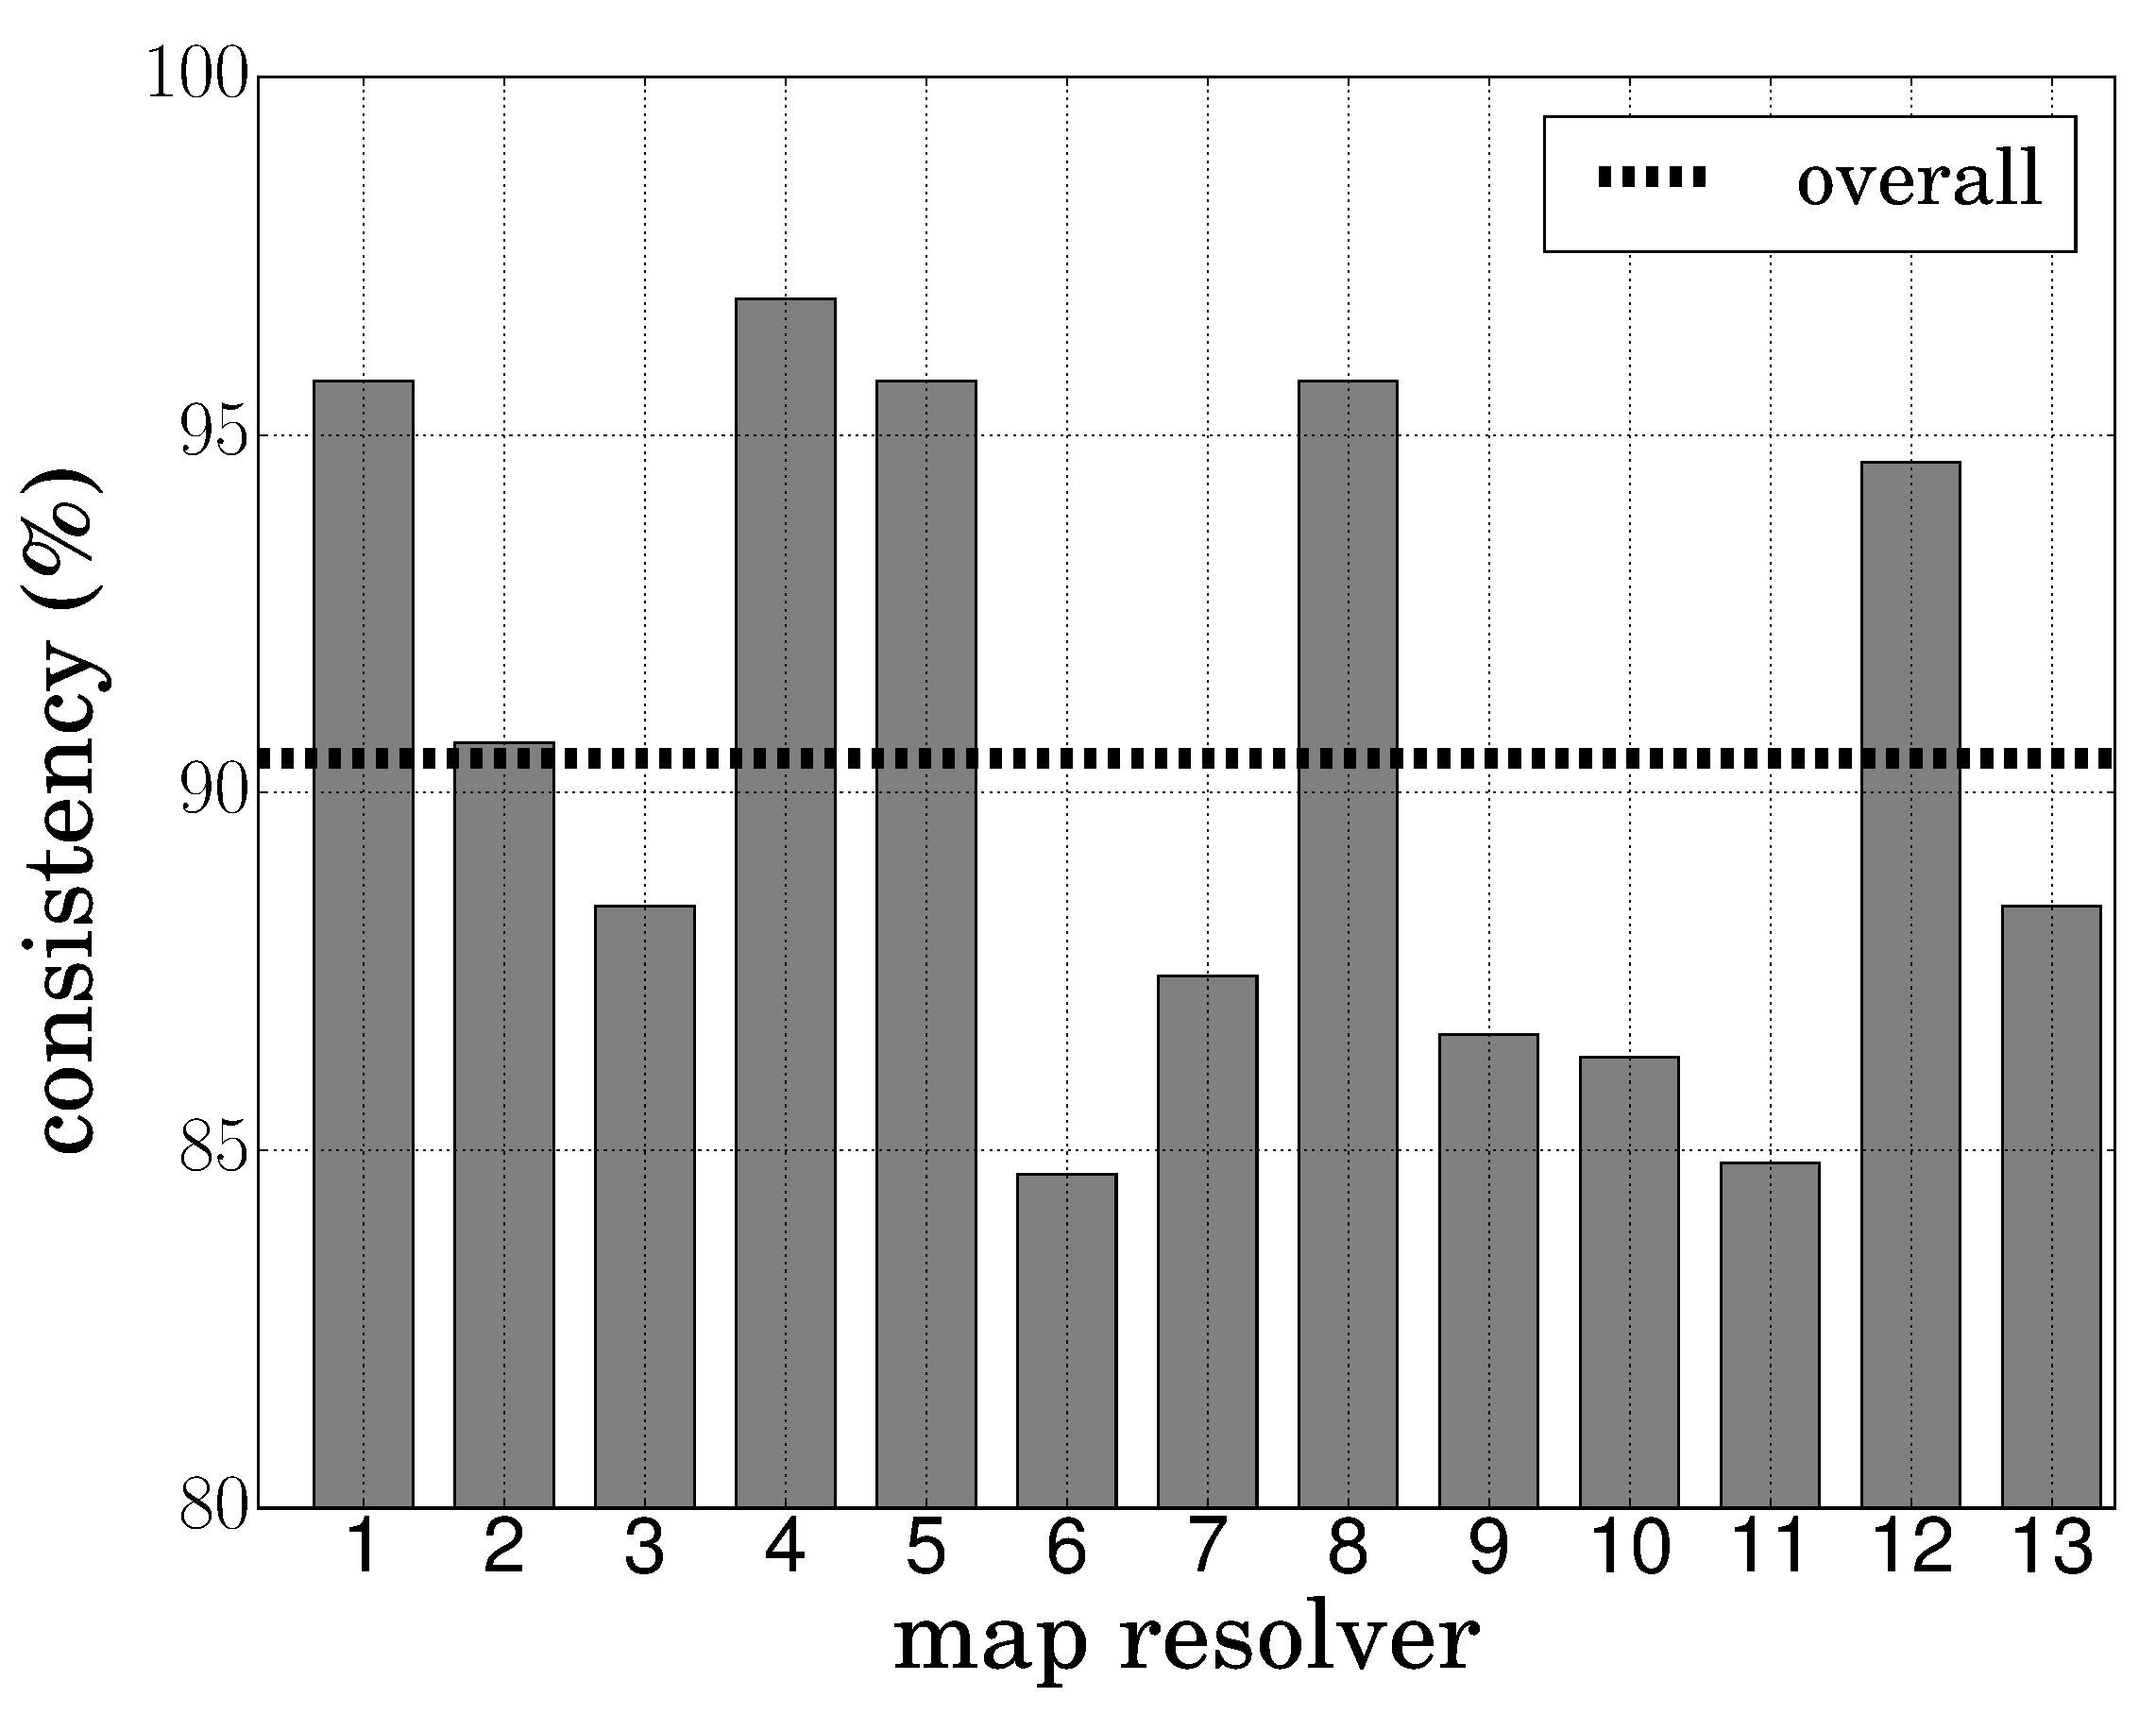
\includegraphics[width=0.7\textwidth]{Pics/Percentage_consistency_13MR_VP.eps}
	\caption{Overall consistency by VP from the different Map-Resolvers.}
	\label{fig:Percentage_consistency_13MR_VP}
\end{figure}
%-< END FIGURE >--------------------------------------------------------------------

The overall percentage of consistency by VP for the whole experiment dataset is 90.48\%, presented by the dotted line in Fig.\ref{fig:Percentage_consistency_13MR_VP}, which indicates that the Map-Replies received at different VPs from the same MR are highly consistent. Yet, we can also observe that different MRs show some deviations from the overall consistency by VP, reflecting the fact that certain MRs send the same Map-Reply to all VPs, but some do not. The deviation among different MRs is however limited (less than 12.23\%). Therefore, we can certainly state that the mapping system shows generally a high degree of consistency by VP but presents a non-negligible amount of inconsistencies (9.52\%). In the rest of this section, following the same approach as for the consistency by MR, we go deeper in this issue, exploring the reasons why some observations exhibit inconsistency by VP.

%-< FIGURE >--------------------------------------------------------------------
\begin{figure}[!t]
	\centering
	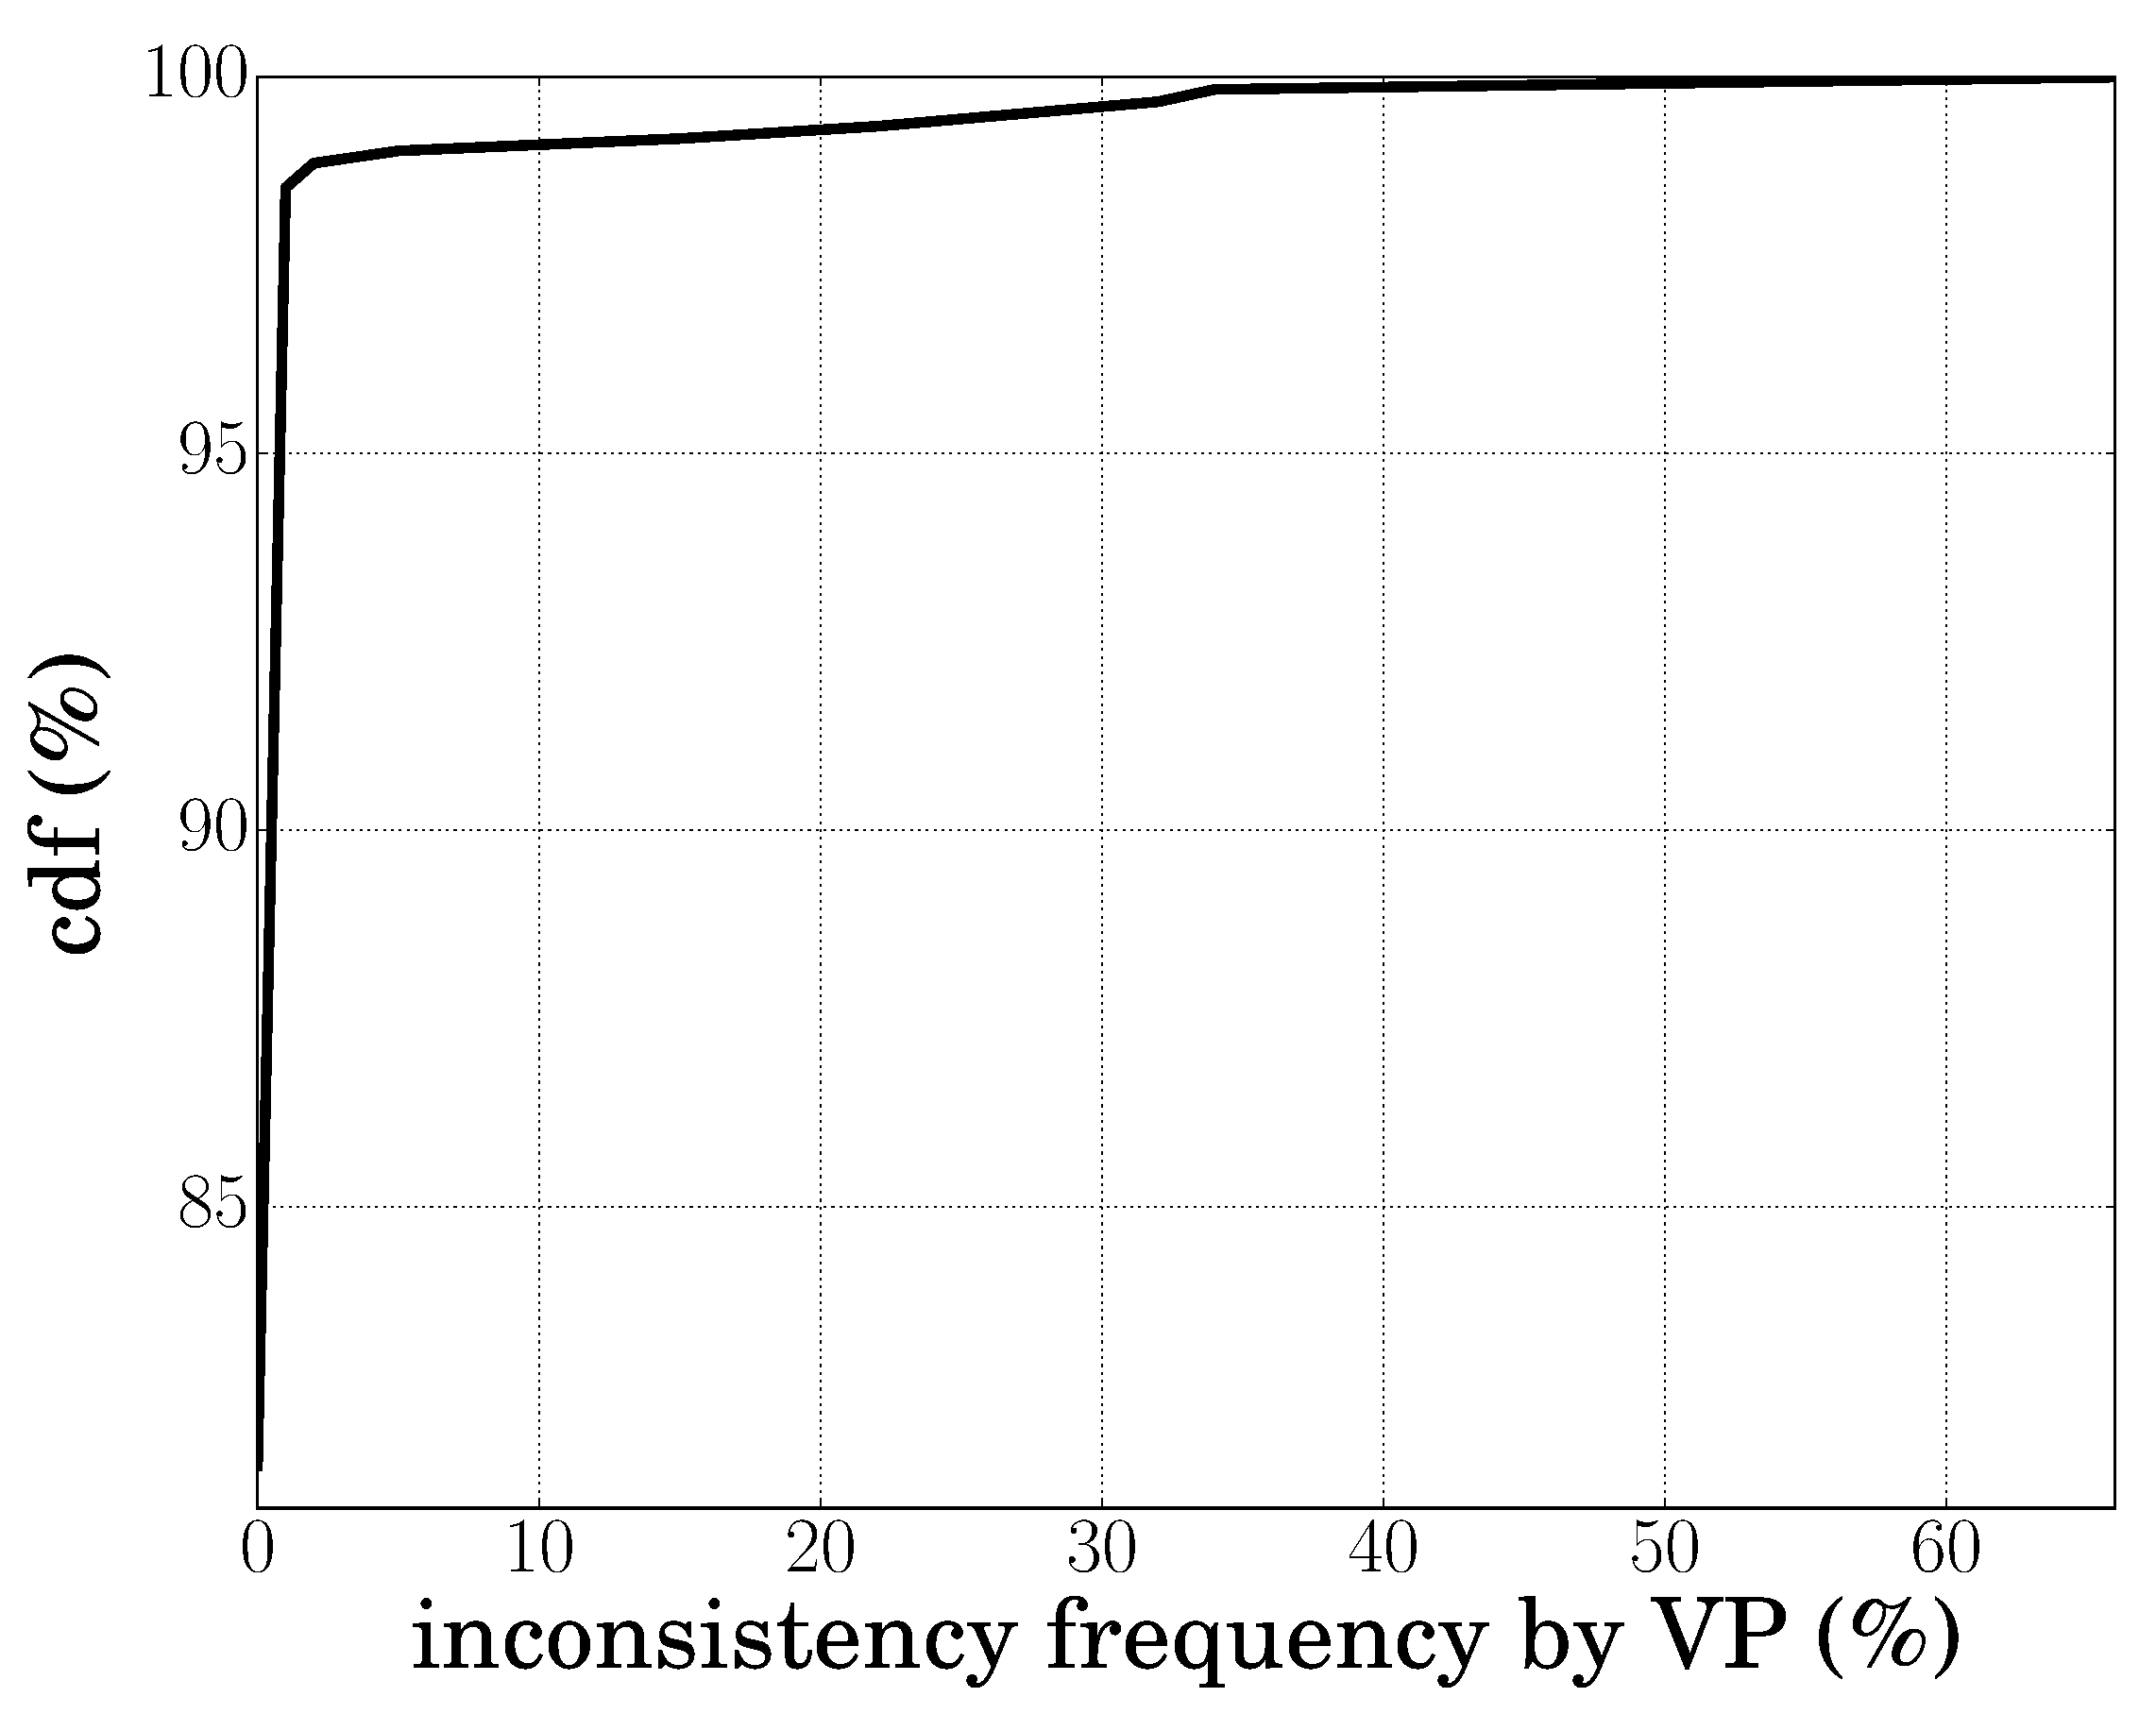
\includegraphics[width=0.7\textwidth]{Pics/cdf_incons_occur_VP.eps}
	\caption{Cumulative Distribution Function of inconsistency frequency by VP. X-axis is inconsistency frequency by VP, indicating the ratio of inconsistency occurrence for each <$EID, MR, *$> tuple over total experiment number.}
	\label{fig:cdf_incons_occur_VP}
\end{figure}
%-< END FIGURE >--------------------------------------------------------------------

Fig.\ref{fig:cdf_incons_occur_VP} shows the CDF of the inconsistency frequency by VP: $f_{<EID, MR, *>}$, i.e., the probability of inconsistency frequency for all <$EID,MR,*$> tuples, by using the following definition: 
\begin{equation}
f_{<EID, *, VP>} = \frac{\text{\# Inconsistencies by VP}}{\text{\# Experiments}}\times100\%.
\end{equation}
Like for the explanation for Fig.~\ref{fig:cdf_incons_occur_MR}, here an inconsistency frequency by VP of 0\% means that all Map-Replies received by all of the VPs from a same MR are totally consistent at every experiment round during the whole experiment campaign, while an inconsistency frequency of 100\% means that at least one of VPs received an inconsistent Map-Reply compared to the other VPs at every experiment round. The probability of consistency by VP (when X-axis is 0\% in Fig.~\ref{fig:cdf_incons_occur_VP}) is similar to that by MR, with a value of 81.57\%. It can be noticed that this percentage is slightly lower than the overall percentage of consistency by VP in Fig.~\ref{fig:Percentage_consistency_13MR_VP}. The reason is that here the inconsistent occurrence with 0\% only includes those EIDs for which all VPs always show consistency, no matter which MR is actually queried. A sharp increase with a growth of 16.97\% % (98.53\% - 81.56\%) 
is found when X-axis is 1\%, which means that although VPs sometimes receive inconsistent Map-Replies at several experiment rounds, the occurrence remains pretty low, hence showing that even by VP  the mapping system exhibits a very high degree of consistency. Differently from the largest inconsistency frequency by MR, which goes up to reaches 100\%, the largest inconsistency frequency by VP is only 66\%. This phenomenon indicates a fact that the Map-Replies received by different VPs are not inconsistent all the time, at least there are one third of observations show that their Map-Replies are totally same. Thus, the consistency by VP is higher than consistency by MR.

To further explore the inconsistency by VP, we then use same metrics as in Sec.~\ref{subsec:mds_consistency_MR}, with the exception that the queried target changes from <$EID, *, VP$> to <$EID, MR, *$> tuples.

The most inconsistent case, 89.06\%, is due to a mix of Negative Map-Reply and LISP Map-Reply, i.e., demand for a same <$EID, MR, *$> tuple, at some VPs receive Negative Map-Reply but at others receive LISP Map-Reply. This is caused by the New Deployment case, but differently from the cause for inconsistency by MR, the reason for inconsistency by VP is probably because of Map-Requests sent by different VPs can not be processed exactly at the same time, due to queuing in the MR. Thus, if the queries are sent during the period of mapping information update, some VPs, whose Map-Requests are processed first will have different Map-Reply Type from the latter ones. Inconsistencies caused by different RLOC sets, i.e., different VPs receive LISP Map-Replies with different RLOCs set from the same MR, also exist, contributing for around 10.94\%. It is probably caused by a combination of the Statistical outliers instability case and the queuing mechanism in MR. As the RLOC sets provided by a MR for some certain EIDs frequently change, and the Map-Requests sent by different VPs need to be processed one by one, it is very possible that the first processed Map-Requests are replied by the different RLOC sets compared to the latter ones. The difference between Map-Replies is probably due to traffic engineering policies, but the further experiments are needed to explore the deeper reasons for such inconsistency.



%-< SECTION >--------------------------------------------------------------------
%\section{LISP-related Discussion and Conclusion}
\section{Summary}
\label{sec:mds_conclusion}
% \begin{itemize}[noitemsep,topsep=0pt]
%     \item Measurements show that the LISP mapping system is stable and consistent over time. 
%     \item Nevertheless, instability and inconsistency are observed but are rare events.
%     \item We developed a new taxonomy to deeper study instability and inconsistency.
%     \item We also provide possible reasons causing the instability and inconsistency, but need future proves.
% \end{itemize}

During the evaluation of LISP mapping system performance, besides the observations about the stability and consistency that we describe in details in the previous sections, we also investigate some interesting LISP-related results. We provide them here so that they can be used to improve LISP performance. We identified that 8.97\% of the LISP-sites leverage on multiple RLOCs in order to be multihomed to the Internet, with an average of 3 distinct locators. Interestingly, when we compare the locators with their Autonomous System Number we found that around 50\% of the locators in multihoming situations belong to different ASes, which indicates that LISP is used to transparently interconnect LISP-sites by the intermediate of multiple ISPs.\footnote{We used the Team Cymru BGP database to associate IP addresses to ASNs (see http://www.team-cymru.org/IP-ASN-mapping.html).} As the control-plane (i.e., MS/MR and mapping system) and the data-plane (i.e., ETR/ITR) are decoupled in LISP, Map-Replies can originate from the LISP-sites directly or from shared utilities constituting the mapping system (i.e., MS/MR). This particularity of LISP is already used in the current deployment, where only 88.8\% of the non-negative Map-Replies are originated directly from their LISP-sites, with the remaining 11.2\% being originated by delegated MSes replying on behalf of the LISP-sites. This allows to reduce the control traffic seen by LISP-sites and help them to scale better.

In addition to mappings, LISP also relies on encapsulation, meaning that with LISP traffic can be transported over IPv4 or IPv6 without requiring end-hosts to be dual-stack. Interestingly, we identified that no less than 8.84\% of the locators are IPv6. However, we have not observed cases where a LISP site was reachable strictly using IPv6 while 82.79\% of sites are reachable only through IPv4. This discrepancy tends to confirm that network operators still lack of confidence being reachable only through IPv6. As a result, the 17.21\% of LISP-sites explicitly using IPv6, always include at least one IPv4 address in order to be reachable.

As a solution to cope with the increase of BGP routing table, traffic engineering, and scalability issues, LISP has been widely deployed on the LISP Beta Network experimental testbed for ten years. To ensure accurate and efficient communications, LISP mapping system should be stable and consistent. However, there is no study evaluating the stability and consistency of LISP mapping system. For such purpose, we continuously measured the LISP Beta Network for seventeen days to assess the mapping system from these two aspects. Measurements show that the LISP mapping system is stable and consistent over time. Nevertheless, instability and inconsistency are observed and for studying them in details we developed a new taxonomy. All in all, instability and inconsistency are rare events. At last, we observe utilization of multi-homing and dual-stack (i.e., IPv4 and IPv6) during the whole experiment and plan to use these results to further improve the LISP performance.